\documentclass{article} % For LaTeX2e
\usepackage{style,times}
\usepackage{hyperref}
\usepackage{url}
%\documentstyle[nips14submit_09,times,art10]{article} % For LaTeX 2.09
\usepackage{graphicx}
\usepackage{amsmath}
\usepackage{enumerate}
\usepackage{subfigure}
\usepackage{amsfonts}
\usepackage{listings}
\usepackage{color}

\usepackage[utf8]{inputenc}

% Default fixed font does not support bold face
\DeclareFixedFont{\ttb}{T1}{txtt}{bx}{n}{12} % for bold
\DeclareFixedFont{\ttm}{T1}{txtt}{m}{n}{12}  % for normal

% Custom colors
\usepackage{color}
\definecolor{deepblue}{rgb}{0,0,0.5}
\definecolor{deepred}{rgb}{0.6,0,0}
\definecolor{deepgreen}{rgb}{0,0.5,0}
\definecolor{Background}{rgb}{0.98,0.98,0.98}
\definecolor{Comments}{rgb}{0,0.63,1}

\usepackage{listings}

% Python style for highlighting
\newcommand\pythonstyle{\lstset{
language=Python,
basicstyle=\ttm,
backgroundcolor=\color{Background},
commentstyle=\color{Comments},
otherkeywords={self,assert,assertEqual},             % Add keywords here
keywordstyle=\ttb\color{deepgreen},
emph={MyClass,__init__},          % Custom highlighting
emphstyle=\ttb\color{deepblue},    % Custom highlighting style
stringstyle=\color{deepred},
frame=tb,                         % Any extra options here
showstringspaces=false            % 
}}


% Python environment
\lstnewenvironment{python}[1][]
{
\pythonstyle
\lstset{#1}
}
{}

% Python for external files
\newcommand\pythonexternal[2][]{{
\pythonstyle
\lstinputlisting[#1]{#2}}}

% Python for inline
\newcommand\pythoninline[1]{{\pythonstyle\lstinline!#1!}}

\title{STA 663: Spring 2017 - Final Project\\Graph-Coupled HMMs for Modeling the Spread of Infection}


\author{
Yimeng Jia \thanks{Our code is maintained in Github Repository, \textcolor{blue}{\url{https://github.com/yimeng-jia/STA663_FinalProject_GCHMM}}}\\
Duke University\\
Durham, NC 27708 \\
\texttt{yimeng.jia@duke.edu} \\
\And
Dewen Xu \\
Duke University \\
Durham, NC 27708 \\
\texttt{dewen.xu@duke.edu} \\
}

\newcommand{\fix}{\marginpar{FIX}}
\newcommand{\new}{\marginpar{NEW}}

\nipsfinalcopy % Uncomment for camera-ready version

\begin{document}

\maketitle

\lstset{
basicstyle=\footnotesize\ttfamily,
frame=L,
breakatwhitespace=false,
language=Matlab,
commentstyle=\color{mygreen},
keywordstyle=\color{blue}}



\begin{abstract}
HMMs (Hidden Markov Models) model independent sequenced or discrete time-series data, and represent long-range dependencies between observations for each data point, mediated via the latent variables. In previous studies, researchers in epidemiology use HMMS to model the spread of infectious disease within a certain social network at the level of entire population over discrete timestamps. However, if researchers are interested in modeling the spread of disease at individual level (interactions among people in a community are considered), the independent assumption between each data sequence does not hold, hence simple HMMs is not appropriate to simulate the generative process. Taking this into consideration, the authors develop Graph-Coupled Hidden Markov Models (GCHMMs) which allows dependencies between state transitions across multiple Hidden Markov Models (HMMs) that properly reflects the spread of infectious disease with effect of individual in a certain group. In our final project, we will implement Gibbs sampler and Generalized Baum-Welch Algorithm for GCHMMs and compare the efficiency and results of two algorithms.
Keywords:  Flu Diffusion, GCHMMs, Gibbs Sampler, Generalized Baum-Welch
\end{abstract}

\section{Introduction}
In medical informatics, one of the important topics is disease diffusion modeling, which helps to take the control of spread of diseases and to provide relevant health advice for people. In the past, due to the limitations of technology, it was difficult to collect the data reflecting the disease spreading at the individual level. However, with the appearance of mobile health apps such as built-in Health apps in apple watch, researchers can get access to the desired data for predicting the disease on an individual level. One related data collection experiment was done by MIT lab: 84 selected undergraduate students who lived in the same dormitory were assigned cell phones with sensors and a designed health App. The sensors supported by Bluetooth could record the interactions among this group of students when any of them were in a circle with a diameter of 1 meter. This group of students were supposed to report their symptoms such as runny nose, and coughing via the health app every day for 107 days.  Unlike the traditional social network data, which relies on self-reported network connections, the cell phone’s sensors guaranteed the completeness of the whole social network throughout the experiment, which reduces the chance of missing data and enhances the robustness of statistical inferences that would be built upon later.	

The two papers we selected to model the flu diffusion in the above situation are Graph-Coupled HMMs for Modeling the Spread of Infection written by \cite{dong2012graph} and Bayesian Models for Heterogeneous Personalized Health Data written by \cite{fan2015bayesian}. Traditional epidemiology research is mainly focused on the infectious simulation on a large population. However, the GCHMMs invented and developed by Dong and Kai allow researchers to model the spread of infectious disease locally within a smaller social network, such as a community or a dormitory. By incorporating a dynamic social network into a coupled HMMs, the GCHMMs can successfully predict health condition of each individual and monitor the path of illness transmission through individuals in a social network, which help researchers to understand how disease is transmitted locally within a network, and to give advice treatment on an individual level.

In CHMMs, the latent state of HMM i at time t is dependent on the latent states of all HMMs in the CHMM at time t-1. In GCHMM, the latent state of HMM i at time t depend on the any number of HMMs that have edges in the graph connected to node n.

GCHMMs (figure 1c) is a dynamic model combining a number of HMMs (figure 1a) together by adding directed edges among hidden states. Each HMM represents one time-series data (a student in our epidemiology model) and its latent/observed  state at time t only depends on the latent/observed state at time t-1. Hidden state is the latent variable indicating whether a student is infectious or not at current time, while observed state is the symptoms behavior. Both the two states are discrete data type in the model. Unlike Coupled-HMMs (figure 1b) which latent state of HMM i at time t is dependent on the latent states of all HMMs at time t-1, in the GCHMM the latent state of HMM i at time t depend on the any number of HMMs that have edges in the graph connected to node n. The edges among different HMMs at different timesteps are described by dynamic network graphs (cloud-shape figures above each time step in figure 1c), describing all the interactions between each consecutive timestamp. For example, during time $t$ to $t+1$, student $x_1$ and student $x_2$ contacts to student $x_3$ which are reflected by the third network graph (node1 and node2 are connected to node3) above time stamp $t+1$.

\begin{figure}[htpb]
\centering
\subfigure[Simple Hidden Markov Model]{
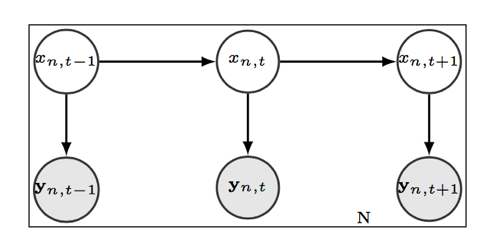
\includegraphics[width=65mm]{HMM.png}
}
\subfigure[Coupled Hidden Markov Model]{
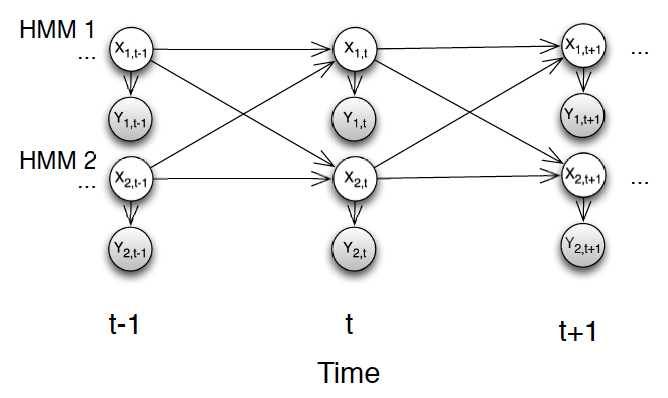
\includegraphics[width=65mm]{CHMM.png}
}
\subfigure[Graph Coupled Hidden Markov Model]{
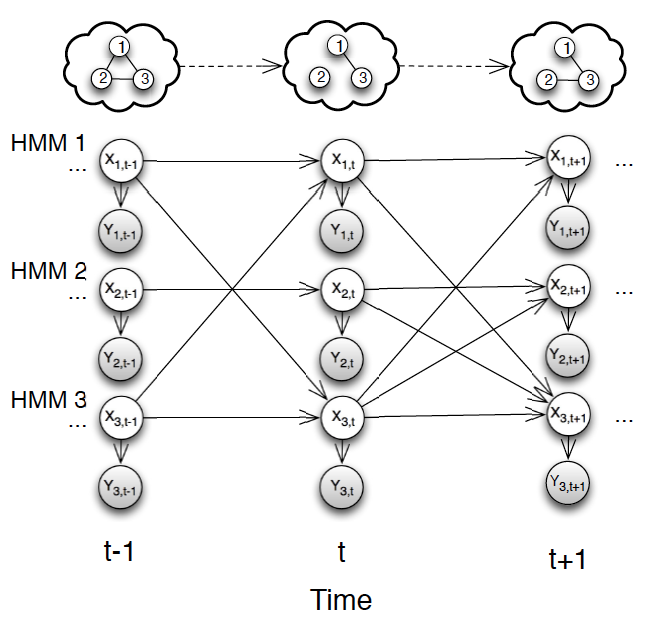
\includegraphics[width=65mm]{GCHMM.png}
}
\caption{Various HMMs}
\label{fig:hmms}
\end{figure}


\paragraph{Notations}
\begin{itemize}
\item $n:1,\ldots,N$ index for each HMMs
\item $t:1,\ldots,T$ index for timestamp
\item $s:1,\ldots,S$ index for symptoms of observation
\item $\gamma$ recovery probability if infectious at pervious time
\item $\alpha$ probability being infected from some one outside networks
\item $\beta$ probability being infected from some one inside networks
\item $x_{n,t} \in \mathcal{X}=\{0,1\}$ the hidden state whether infectious
\item $y_{n,t} \in \mathcal{Y}=\{0,1\}^S$ the symptoms onset
\item $\xi$ hyper parameter for the prior Bernoulli distribution of $x_{n,1}$
\item $\theta_{x_{n,t},s}$ emission probability of symptom $s$ onset
\item $G_t$ the dynamic social network graph between time $t$ and $t+1$
\item $E_t$ the set of edge on $G_t$
\end{itemize}


\section{Generative Model}

\subsection{Probablistic Model}
A coupled hidden Markov model (CHMM) describes the dynamics of a discrete-time Markov process that links together a number of distinct standard hidden Markov models (HMMs). In a standard HMM, the value of the latent state at time $t$ is dependent on only the value of the latent state at last time $t-1$. In contrast, the latent state of GCHMMs at time $t$ in the GCHMMs is dependent on the latent states of a subset of HMMs in the GCHMMs at time $t-1$, where the subset is determined by the graph at time $t-1$. Therefore, the generative model of GCHMMs can be readily stated.

\begin{align*}
\xi&\sim\text{Beta}(a_\xi,b_\xi) \quad &\alpha\sim\text{Beta}(a_\alpha,b_\alpha)\\
\beta&\sim\text{Beta}(a_\beta,b_\beta) \quad  &\gamma\sim\text{Beta}(a_\gamma,b_\gamma)\\
\theta_{0,s}&\sim\text{Beta}(a_0,b_0)\quad &\theta_{1,s}\sim\text{Beta}(a_1,b_1)\\
x_{n,0}&\sim\text{Bernoulli}(\xi)\quad &x_{n,t}\sim\text{Bernoulli}\left(\phi_{n,x_{n'}:(n,n')\in G_t}(\alpha,\beta,\gamma)\right)\\
y_{n,t,s}&\sim\text{Bernoulli}(\theta_{x_{n,t},s})\\
\end{align*}
%
According to the definition of $\xi,\alpha,\beta,\gamma$, they all represent small probabilities so their prior should have a small mean in application. $\theta_{1,s}$ means the symptom appearance probability when got infectious, thus being reasonable to set a higher mean prior. $\theta_{0,s}$ is on the contrary. Notice that the transition probability $\phi_{n,x_{n'}:(n,n')\in G_t}(\alpha,\beta,\gamma)$ here is a function of three parameters. As the notations, this term is a little subtle because of its dependence on previous infection state. The exact definition will be introduced in the factor graph section.

\subsection{Transition Function}
According to Figure \ref{fig:hmms}(c), the bayesian network has two type of factors (conditional probability), emission probability function $\phi_{n,t,y|x,s}(y_{n,t,s}|x_{n,t})=p(y_{n,t,s}|x_{n,t})$ and transition probability function $\phi_{n,t-1,t}(x_{n,t-1},x_{n',t-1:(n',n)\in E_{t-1}},x_{n,t})=p(x_{n,t}|x_{n,t-1},x_{n',t-1:(n',n)\in E_{t-1}})$. Based on the generative model, the factors have the following expression.
\begin{align*}
\phi_{n,t,y|x,s}(y_{n,t,s}|x_{n,t})&=\theta_{x_{n,t},s}^{y_{n,t,s}}(1-\theta_{x_{n,t},s})^{y_{n,t,s}}\\
\phi_{n,t-1,t}(x_{n,t-1},x_{n',t-1:(n',n)\in E_{t-1}},x_{n,t})&=\left\{ \begin{matrix} 
      \gamma & \text{if $x_{n,t-1}=1,x_{n,t}=0$} \\
      1-\gamma &  \text{if $x_{n,t-1}=1,x_{n,t}=1$} \\
      1-(1-\alpha)(1-\beta)^{\sum_{n':(n',n)\in E_{t-1}}x_{n',t-1}} & \text{if $x_{n,t-1}=0,x_{n,t}=1$}\\
      (1-\alpha)(1-\beta)^{\sum_{n':(n',n)\in E_{t-1}}x_{n',t-1}} & \text{if $x_{n,t-1}=0,x_{n,t}=0$}\\
   \end{matrix}\right.\\
\end{align*}
With the factor definition, the standard bayesian network can be easily represented to factor graph Figure \ref{fig:fgchmm}. The factor graph is still shown by template formulation; each template represents a patient while the interaction is captured by transition factor. In fact, during the later EM algorithm, all parameters are unknown so that we can put parameter node containing $\alpha,\beta,\gamma$ at the top of the current whole graph, having connection edge with all transition factors. Similarly, parameter nodes $\xi$ and $\theta_0,\theta_1$ can be added in the same way. For simplicity, we did not include them in our factor graph, though this parameter node trick is a commonly used method.

\begin{figure}[t]
\centering
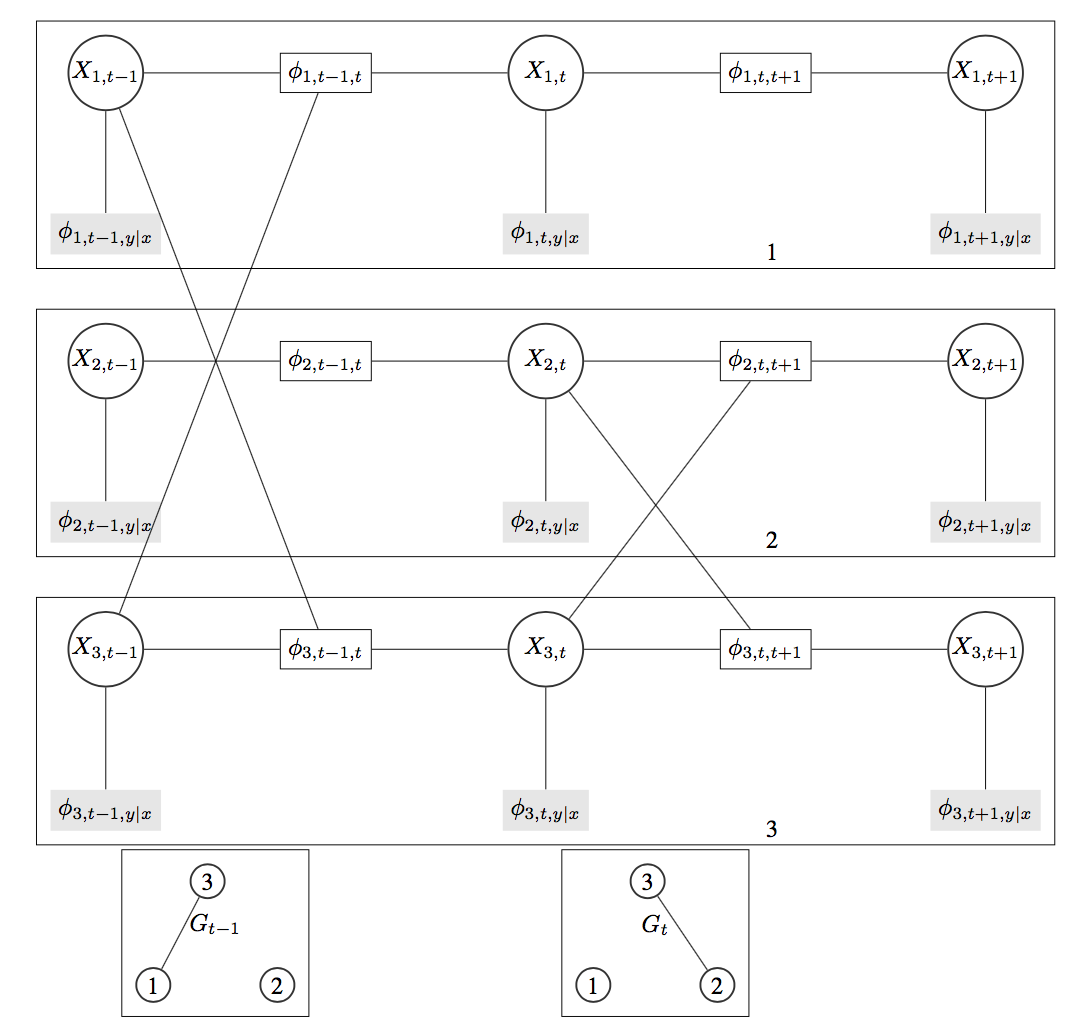
\includegraphics[width=100mm]{EM_GCHMM.png}
\caption{Factor Graph of GCHMMs}
\label{fig:fgchmm}
\end{figure}

\section{Gibbs Sampling Algorithm}

\subsection{Update latent sequence $x_{1:D}$}
We can easily write the joint likelihood as follows.
\begin{align*}
P(\mathbf{Y}_{n,1:T}, \mathbf{X}_{n,0:T}) 
&= \boldsymbol{\pi}_0(X_{n,0})P(X_{n,1}|X_{n,0},\phi)P(Y_{n,1}|X_{n, 1}, \theta)\\
&\prod_{t = 2}^{T} P(X_{n,t}|X_{n, t-1}, X_{n': \left \{ n',n \right \}\in E_{t-1},t-1}, \phi)P(Y_{n,t}|X_{n, t}, \theta)
\end{align*}
Thus, the posterior for $X$.
\begin{align*}
X_{n,t+1}|{X,Y} \setminus X_{n,t+1;\mu} \sim \text{Categorical}\left( \frac{P(X_{n,t+1})}{\sum_{x}P(X_{n,t+1=x})}\right) \\
%Y_{n,t,s} &\sim\\
\end{align*}

\subsection{Update parameters in transition distribution}
The Baysian model is not conjugate for parameters, so we introduce an auxiliary latent variable $R$ to make our model approximately conjugate. 
The augumented variable $R$ means 
\begin{align*}
R_{n,t} \sim \text{Categorical}\left( \frac{\alpha,\beta, ..., \beta }{\alpha +\beta\sum_{n'}1_{(n',n)\in E_{t}\cap X_{n',t} =1} } \right)
\end{align*}

$\alpha | X \sim \text{Beta}( a + \sum_{n,t}1_{\left \{ R_{n, t=1} \right \}},b+ \sum_{n,t:X_{n,t=0}}1- \sum_{n,t}1_{\left \{ R_{n,t=1} \right \}})$

$\beta | X \sim \text{Beta}({a}' + \sum_{n,t}1_{\left \{R_{n,t >1}\right \}}, {b}' + \sum_{n,t:X_{n,t=0;n'}}1_{(n',n) \in E_{t} \bigcap X_{n', t} =1  - \sum_{n,t}1_{\{ \{ R_{n,t>1}} \}})$

$\gamma| X \sim \text{Beta}(a'' + \sum_{n,t:X_{n,t=1}}1_{\left \{ X_n,t+1=0 \right \}},\ b''+ \sum_{n,t:X_{n,t=1}}1 -\sum_{n,t:X_n,t=1}
1_{\left \{ X_{n,t+1=0} \right \}})$

\subsection{Update parameters in emission distribution}
$p(\boldsymbol{\theta_{k,s}}| Y) \sim \text{Beta}(a_k + \sum \mathbb{I}_{Y_{n,t,s}=1, X_{n,t}=k}, b_k + + \sum \mathbb{I}_{Y_{n,t,s}=1, X_{n,t}=k})$, for $k = 0, 1$

\section{Generalized Baum-Welch (GBW) Algorithm}

Two main contributions in Fan's generalized the Baum-Welch Algorithm for bounded GCHMMs are included in this section: the first is to use belief propagation to derive the forward-backward algorithm that is parallel in standard HMMs; the second is to apply an approximate EM algorithm for parameter estimation. 

\subsection{Single Node Belief Propagation Rules: Forward-backward}
Notice that even if the Bayesian network Figure is not exactly a directed polytree (cyclic path exists if direction is omitted), marginals inference on each hidden node can still be approximated by belief propagation by factor graph for the sake of efficiency. In this section, we will show the derivation of the single node belief probation rules on Figure \ref{fig:fgchmm}. Denote the message passing to the child, i.e. from $x_{m,t-1}$ to $x_{n,t}$ as $\pi_{x_{m,t-1}}(x_{n,t})$, and the message to parent, i.e. from $x_{k,t+1}$ to $x_{n,t}$ as $\lambda_{x_{k,t+1}}(x_{n,t})$. Then, the belief or probability distribution passed with all evidence shown is denoted as $BEL(x_{n,t})=P(x_{n,t}|Y)$. Our derivation is based on Pearl's belief propagation algorithm \cite{pearl1988probabilistic}. All $\propto$ in the following imply the term should be normalized to 1 as a probability distribution.

It has been proved that belief propagation on standard HMMs is equivalent to forward-backward algorithm. It is still similar to write down forward-backward framework in our coupled case. However, the update step for message passing here is a little complicated since the single node dependence is generalized to multi-nodes. Here we need the assumption maximum degree of all $G_t$s is bound by $M$. In this case, the update of sum-product for message can be computed efficient, i.e. $\mathcal{O}(2^M)$ at each iteration.

\begin{align*}
\pi^{(i)}(x_{n,t})&=\sum_{x_{n,t-1},x_{n',t-1:(n'n)\in E_t}}\phi_{n,t-1,t}\prod_{n\cup\{n':(n',n)\in E_{t-1}\}}\pi_{x_{n,t}}^{(i)}(x_{\cdot,t-1})\\
\lambda^{(i)}(x_{n,t})&=\prod_{s=1}^S\lambda_{y_{n,t,s}}(x_{n,t})\prod_{n\cup\{n':(n,n')\in E_t\}}\lambda_{x_{\cdot,t+1}}^{(i)}(x_{n,t})\\
BEL^{(i)}(x_{n,t})&\propto \pi^{(i)}(x_{n,t})\lambda^{(i)}(x_{n,t})
\end{align*}
where
\begin{align*}
\pi_{x_{n,t}}(x_{\cdot,t-1})&=p(x_{n,t}|x_{\cdot,t-1})\text{ and }\lambda_{x_{\cdot,t+1}}(x_{n,t})=p(x_{\cdot,t+1}|x_{n,t}).
\end{align*}
 
\paragraph{Updating $\lambda$}
\begin{align*}
\lambda_{x_{n,t}}^{(i+1)}(x_{n,t-1})&\propto\sum_{x_{n,t}}\lambda^{(i)}(x_{n,t})\sum_{x_{n',t-1}:(n',n)\in E_{t-1}}\phi_{n,t-1,t}\prod_{n':(n',n)\in E_{t-1}}\pi_{x_{n,t}}^{(i)}(x_{\cdot,t-1})\\
\lambda_{x_{n,t}}(x_{n,t-1}=1)&\propto\sum_{x_{n,t}}\lambda(x_{n,t})\gamma^{\mathbb{I}_{x_{n,t}=0}}(1-\gamma)^{\mathbb{I}_{x_{n,t}=1}}\\
\lambda_{x_{n,t}}(x_{n,t-1}=0)&\propto\sum_{x_{n,t}}\lambda(x_{n,t})\sum_{x_{n',t-1}:(n',n)\in E_{t-1}}\left[1-(1-\alpha)(1-\beta)^{\sum_{n':(n',n)\in E_{t-1}}x_{n',t-1}}\right]^{\mathbb{I}_{x_{n,t}=1}}\\
&\left[(1-\alpha)(1-\beta)^{\sum_{n':(n',n)\in E_{t-1}}x_{n',t-1}}\right]^{\mathbb{I}_{x_{n,t}=0}}\prod_{n':(n',n)\in E_{t-1}}\pi_{x_{n,t}}(x_{\cdot,t-1})\\
\lambda_{x_{n,t}}^{(i+1)}(x_{n',t-1})&\propto\sum_{x_{n,t}}\lambda^{(i)}(x_{n,t})\sum_{x_{n,t-1},x_{n'',t-1}\neq x_{n',t-1}:(n'',n)\in E_{t-1}}\phi_{n,t-1,t}\prod_{n\cup\{n''\neq n':(n'',n)\in E_{t-1}\}}\pi_{x_{n,t}}^{(i)}(x_{\cdot,t-1})
\end{align*}

\paragraph{Updating $\pi$}
\begin{align*}
\pi_{x_{n,t+1}}^{(i+1)}(x_{n,t})&\propto \prod_{s=1}^S\lambda_{y_{n,t,s}}(x_{n,t})\prod_{n':(n,n')\in E_t}\lambda_{x_{\cdot,t+1}}^{(i)}(x_{n,t})\pi^{(i)}(x_{n,t})=\frac{BEL^{(i)}(x_{n,t})}{\lambda_{x_{n,t+1}}^{(i)}(x_{n,t})}\\
\pi_{x_{n',t+1}}^{(i+1)}(x_{n,t})&\propto \prod_{s=1}^S\lambda_{y_{n,t,s}}(x_{n,t})\prod_{n\cup\{n''\neq n':(n,n'')\in E_t\}}\lambda_{x_{\cdot,t+1}}^{(i)}(x_{n,t})\pi^{(i)}(x_{n,t})=\frac{BEL^{(i)}(x_{n,t})}{\lambda_{x_{n',t+1}}^{(i)}(x_{n,t})}\\
\pi_{y_{n,t,s}}^{(i+1)}(x_{n,t})&\propto \prod_{s'\neq s}\lambda_{y_{n,t,s'}}(x_{n,t})\prod_{n\cup\{n':(n,n')\in E_t\}}\lambda_{x_{\cdot,t+1}}^{(i)}(x_{n,t})\pi^{(i)}(x_{n,t})=\frac{BEL^{(i)}(x_{n,t})}{\lambda_{y_{n,t,s}}^{(i)}(x_{n,t})}
\end{align*}

\paragraph{Boundary Conditions}
\begin{itemize}
\item Root nodes, i.e. $x_{n,0}$. Let $\pi$ be the prior distribution, i.e. $\pi(x_{n,0})=\xi^{x_{n,0}}(1-\xi)^{1-x_{n,0}}$. 
\item Evidence nodes, i.e. $y_{n,t,s}$
\begin{align*}
\lambda(y_{n,t,s})&=(\mathbb{I}_{y_{n,t,s}=0},\mathbb{I}_{y_{n,t,s}=1}) \\
\pi(y_{n,t,s})&=\sum_{x_{n,t}}\phi_{n,t,y|x,s}(y_{n,t,s}|x_{n,t})\pi_{y_{n,t,s}}(x_{n,t})\\
BEL(y_{n,t,s})&\propto \lambda(y_{n,t,s})\pi(y_{n,t,s})\\
\lambda_{y_{n,t,s}}(x_{n,t})&\propto \sum_{y_{n,t,s}}\lambda(y_{n,t,s})\phi_{n,t,y|x,s}(y_{n,t,s}|x_{n,t})=\mathbb{I}_{y_{n,t,s}=0}(1-\theta_{x_{n,t},s})+\mathbb{I}_{y_{n,t,s}=1}\theta_{x_{n,t},s}
\end{align*}
\item Initialization, all message from variable nodes to factor nodes, such as $\pi_{x_\cdot}(x_\cdot),\lambda_{x_\cdot}(x_\cdot)$, can be set all 1s. Actually, random initialization would affect much of the result because they all will be washed out after a few iterations.
\end{itemize}

\subsection{Message Passing for Approximate EM Algorithm}
In this section, we will put forward two algorithms for parameter learning, particularly in the generalized Baum-Welch Algorithm for GCHMMs. Gibbs sampling algorithm is another widely investigated in this phrase \cite{dong2012graph}. A comparison between the two algorithms will be discussed in the experiment section.

\subsubsection{E-step}
\begin{align*}
\Pr(X,Y;\Theta)&=\prod_{n=1}^N\left\{p(x_{n,0};\xi)\left(\prod_{s=1}^S\phi_{n,0,y|x,s}\right)\prod_{t=1}^T\left[\phi_{n,t-1,t}\left(\prod_{s=1}^S\phi_{n,t,y|x,s}\right)\right]\right\}\\
\log\Pr(X,Y;\Theta)&=\sum_{n=1}^N\left\{\log p(x_{n,0};\xi)+\sum_{t=1}^T\log\phi_{n,t-1,t}+\sum_{t=1}^T\sum_{s=1}^S\log\phi_{n,t,y|x,s}\right\}\\
Q(\Theta,\Theta^{old})&=\sum_{X}\sum_{n=1}^N\left\{x_{n,0}\log\xi+(1-x_{n,0})\log(1-\xi)+\sum_{t=1}^T\log\phi_{n,t-1,t}+\sum_{t=1}^T\sum_{s=1}^S\log\phi_{n,t,y|x,s}\right\}\Pr(X|Y,\Theta^{old})
\end{align*}

\subsubsection{Exact M-step}
\begin{align}
\frac{\partial Q(\Theta,\Theta^{old})}{\partial\xi}&=\sum_{x_{1:N,0}\in\{0,1\}^N}\left(\frac{\sum_{n=1}^Nx_{n,0}}{\xi}-\frac{\sum_{n=1}^N(1-x_{n,0})}{1-\xi}\right)p(x_{1:N,0}|Y,\Theta^{old})=0\\
\Rightarrow \xi &= \frac{\sum_{x_{1:N,0}\in\{0,1\}^N}\left(\sum_{n=1}^Nx_{n,0}\right)p(x_{1:N,0}|Y,\Theta^{old})}{N}=\frac{\sum_{n=1}^N\mathbb{E}[x_{n,0}]}{N}
\end{align}

\begin{align*}
\frac{\partial Q(\Theta,\Theta^{old})}{\partial \theta_{0,s}}=0\Rightarrow \theta_{0,s}&=\frac{\sum_{x_{1:N,1:T}\in\{0,1\}^{N^2}}\left(\sum_{n=1}^N\sum_{t=1}^Ty_{n,t,s}\mathbb{I}_{x_{n,t=0}}\right)p(X|Y,\Theta^{old})}{\sum_{x_{1:N,1:T}\in\{0,1\}^{N^2}}\left(\sum_{n=1}^N\sum_{t=1}^T\mathbb{I}_{x_{n,t=0}}\right)p(X|Y,\Theta^{old})}
\end{align*}
Similarly, $\theta_{1,s}=\frac{\sum_{x_{1:N,1:T}\in\{0,1\}^{N^2}}\left(\sum_{n=1}^N\sum_{t=1}^Ty_{n,t,s}\mathbb{I}_{x_{n,t=1}}\right)p(X|Y,\Theta^{old})}{\sum_{x_{1:N,1:T}\in\{0,1\}^{N^2}}\left(\sum_{n=1}^N\sum_{t=1}^T\mathbb{I}_{x_{n,t=1}}\right)p(X|Y,\Theta^{old})}$

\begin{align*}
\frac{\partial Q(\Theta,\Theta^{old})}{\partial\gamma}=0\Rightarrow \gamma=\frac{\sum_{x_{1:N,1:T}\in\mathcal{X}^{N^2}}\left(\sum_{n=1}^N\sum_{t=2}^T\mathbb{I}_{x_{n,t-1}=1,x_{n,t}=0}\right)p(X|Y,\Theta^{old})}{\sum_{x_{1:N,1:T}\in\mathcal{X}^{N^2}}\left(\sum_{n=1}^N\sum_{t=2}^T\mathbb{I}_{x_{n,t-1}=1}\right)p(X|Y,\Theta^{old})}
\end{align*}

Notice that it does not matter if we change the $p(X|Y,\Theta^{old})$ to $\Pr(X,Y|\Theta^{old})$. Conditions $\frac{\partial Q(\Theta,\Theta^{old})}{\partial\alpha}=0$ and $\frac{\partial Q(\Theta,\Theta^{old})}{\partial\beta}=0$ can be further derived for the iteration step for parameters estimation by EM. However, except for $\xi$, the exact computation complexity of other parameters iteration step is an intractable message passing, exponentially increasing with $N$ or $N^2$. 

\subsubsection{Approximate M-step}
If we approximate $P(X|Y,\Theta^{old})=\prod_{n,t}p(x_{n,t}|Y,\Theta^{old})$ as a fully factorized form, then all the M-step for $\theta$ would be allowed to update easily, because $p(x_{n,t}|Y,\Theta^{old})$ (i.e. $BEL(x_{n,t})$) can be computed by forward-backward algorithm derived before.
\begin{align}
\theta_{0,s}&=\frac{\sum_{n=1}^N\sum_{t=1}^Ty_{n,t,s}\mathbb{E}[1-x_{n,t}]}{\sum_{n=1}^N\sum_{t=1}^T\mathbb{E}[1-x_{n,t}]}\\
\theta_{1,s}&=\frac{\sum_{n=1}^N\sum_{t=1}^Ty_{n,t,s}\mathbb{E}[x_{n,t}]}{\sum_{n=1}^N\sum_{t=1}^T\mathbb{E}[x_{n,t}]}
\end{align}

Updating for $\gamma,\alpha,\beta$ is tricky here. First, we first introduce the approximation for $\gamma$ which will make the two later parameters more understandable. Even if the full factorization assumption holds, the update step for $\gamma$ associates two successive variables $x_{n,t-1}$ and $x_{n,t}$. A natural idea is to use Monte Carlo method to sample $\{\tilde{x}_{1:N,1:T}\}\in \mathcal{X}^{N^2}$ from $P(X|Y,\Theta^{old})=\prod_{n,t}p(x_{n,t}|Y,\Theta^{old})$. Then we count the number that event $x_{n,t-1}=1,x_{n,t}=0$ happens. For simplicity, we can directly assign the simulated sample by Bayesian decision strategy according to each $p(x_{n,t}|Y,\Theta^{old})$ instead of sampling. That is to say, we only need to set the sample $x_{n,t}=\arg\max_{\tilde{x}_{n,t}=\{0,1\}}p(x_{n,t}|Y,\Theta^{old})$. Therefore, the update for $\gamma$ is straightforward.
\begin{align}
\gamma&=\frac{\sum_{n=1}^N\sum_{t=1}^{T}\mathbb{I}_{\tilde{x}_{n,t-1}=1,\tilde{x}_{n,t}=0}}{\sum_{n=1}^N\sum_{t=1}^{T}\mathbb{E}[x_{n,t-1}]}\approx\frac{\sum_{n=1}^N\sum_{t=1}^{T}\mathbb{I}_{\tilde{x}_{n,t-1}=1,\tilde{x}_{n,t}=0}}{\sum_{n=1}^N\sum_{t=1}^{T}\mathbb{I}_{\tilde{x}_{n,t-1}=1}}
\end{align}

The same trick can be applied to update $\alpha,\beta$. However, one more trick needed here. Denote $\tau_i=(1-\alpha)(1-\beta)^i$; then apparently $\alpha=1-\tau_0$. Then the update step for $\alpha$ is similar as $\gamma$.
%
\begin{align}
\alpha &= \frac{\sum_{n=1}^N\sum_{t=1}^{T}\mathbb{I}_{\tilde{x}_{n,t-1}=0,\tilde{x}_{n,t}=1}\mathbb{I}_{\sum_{n':(n,n')\in E_{t-1}}\tilde{x}_{n',t-1}=0}}{\sum_{n=1}^N\sum_{t=1}^{T}\mathbb{E}[1-x_{n,t-1}]} \nonumber \\
	   &\approx\frac{\sum_{n=1}^N\sum_{t=1}^{T}\mathbb{I}_{\tilde{x}_{n,t-1}=0,\tilde{x}_{n,t}=1}\mathbb{I}_{\sum_{n':(n,n')\in E_{t-1}}\tilde{x}_{n',t-1}=0}}{\sum_{n=1}^N\sum_{t=1}^{T}\mathbb{I}_{\tilde{x}_{n,t-1}=0}}
\end{align}
%
Following the trick of $\alpha$, we can easily update $\tau_i,i=1,...,M$. 
%
\begin{align*}
\tau_i &= \frac{\sum_{n=1}^N\sum_{t=1}^{T}\mathbb{I}_{\tilde{x}_{n,t-1}=0,\tilde{x}_{n,t}=0}\mathbb{I}_{\sum_{n':(n,n')\in E_{t-1}}\tilde{x}_{n',t-1}=i}}{\sum_{n=1}^N\sum_{t=1}^{T}\mathbb{E}[1-x_{n,t-1}]} \\
	   &\approx\frac{\sum_{n=1}^N\sum_{t=1}^{T}\mathbb{I}_{\tilde{x}_{n,t-1}=0,\tilde{x}_{n,t}=0}\mathbb{I}_{\sum_{n':(n,n')\in E_{t-1}}\tilde{x}_{n',t-1}=i}}{\sum_{n=1}^N\sum_{t=1}^{T}\mathbb{I}_{\tilde{x}_{n,t-1}=0}}
\end{align*}
%
Obviously, $\beta=1-\left(\frac{\tau_i}{1-\alpha}\right)^{\frac{1}{i}}$, thus meaning we have $M$ estimations for $\beta$s. How to combine these $\beta$s to obtain a better estimation may vary in different applications. So the below algebra average can be adjusted under various circumstances.
\begin{align}
\beta=1-\frac{1}{M}\sum_{i=1}^M\left(\frac{\tau_i}{1-\alpha}\right)^{\frac{1}{i}} .
\end{align}

To sum up, we have our generalized Baum-Welch Algorithm, also called approximate EM Belief propagation(AEMBP), for GCHMMs.
\begin{enumerate}[(I)]
\item $\Theta^{(0)}$ initialization;
\item Run one iteration forward-backward algorithm on $\Theta^{old}$ to obtain $p(x_{n,t}|Y,\Theta^{old})$;
\item Update $\Theta^{new}$ based on equation (2)-(7);
\item If converge, break; else back to (II).
\end{enumerate}

\section{Experimental Results and Comparative Analysis}

\subsection{Application to Real Data Set}

\paragraph {Latent States Prediction} With the dynamic social network data $G_{84\times84\times107}$,  we run the data on two algorithm Generalized BW (GBW) and Gibbs sampling under two cases, with parameter unknown. Both algorithms will only take $Y$ but not $X$ as arguments but will predict an $X$. To observe the performance on real data set, we construct heat maps of the predicted latent states (picture on the middle and right) and compare it with the true latent states (picture on the left). Redness indicates that the student (on the y-axis) get infected on a particular day (x-axis); blueness indicate no infection; and whiteness indicate that the probability of getting infected is 0.5. Overall, Gibbs sampler and Generalized Baum-Welch algorithm achieve very similar predictions of the latent states as the real case, except a few whiteness at the end of an infection line, indicating that the models are uncertain whether the infected student is ready to recover. This makes sense in the real situation because sometimes doctors are unsure when students should be diagnosed as completely recovered at the end of an infection period. Overall, both algorithms achieve comparable performance.

\begin{figure*}[h]
\hspace{-3cm}
\begin{tabular}{ccc}
\subfigure[True Latent States]{
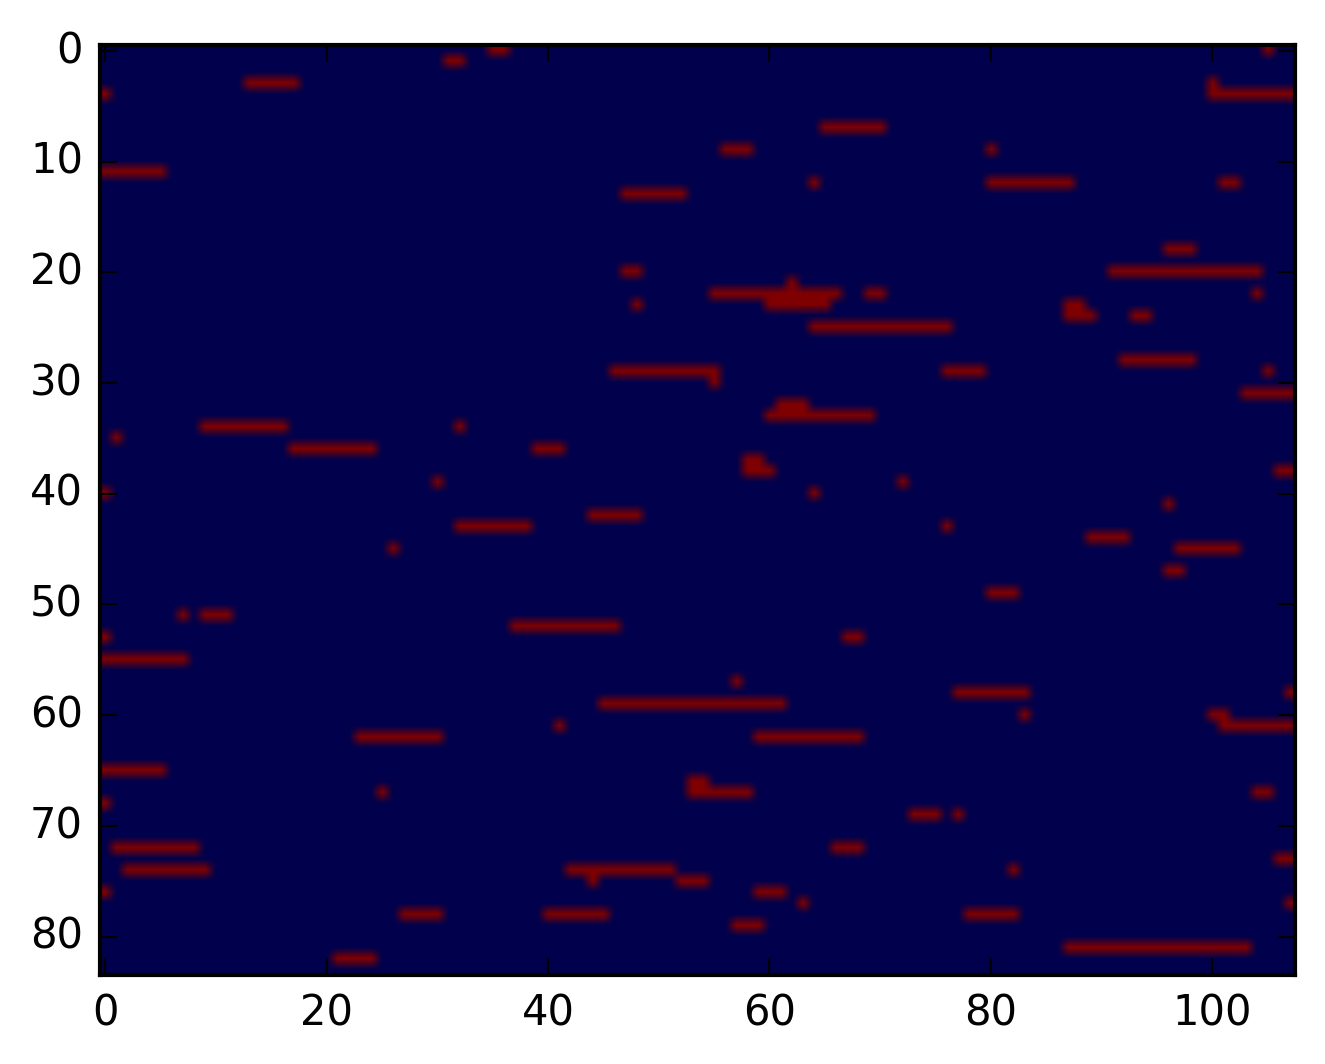
\includegraphics[width=60mm]{true.png}
} &
\subfigure[Predicted Latent States from Gibbs]{
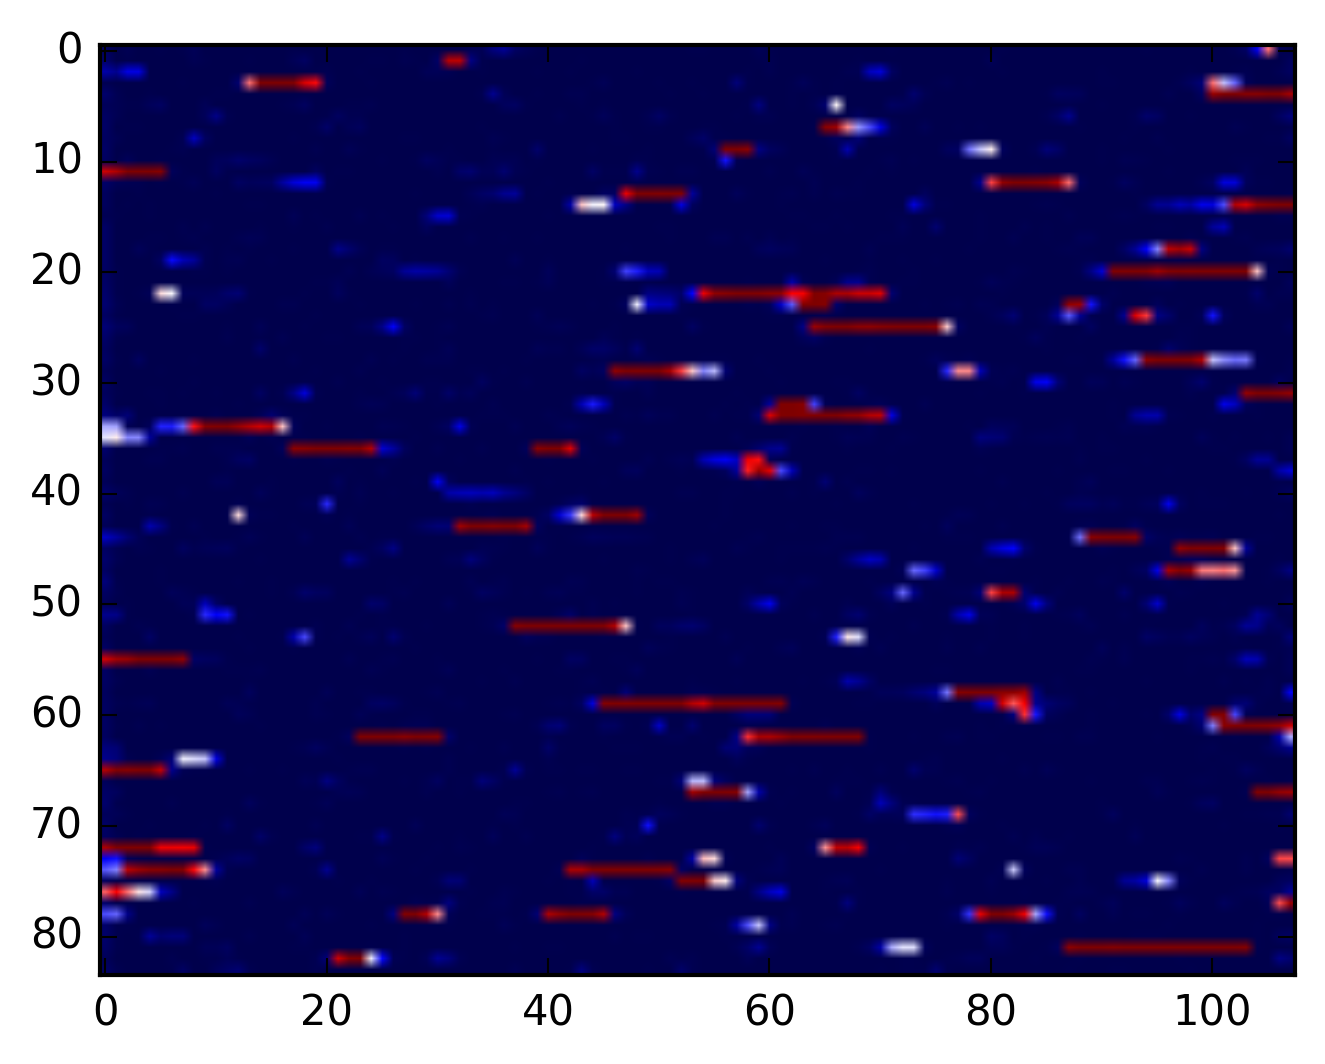
\includegraphics[width=60mm]{predicted.png}
} &
\subfigure[Predicted Latent States from Approx. EM B-W]{
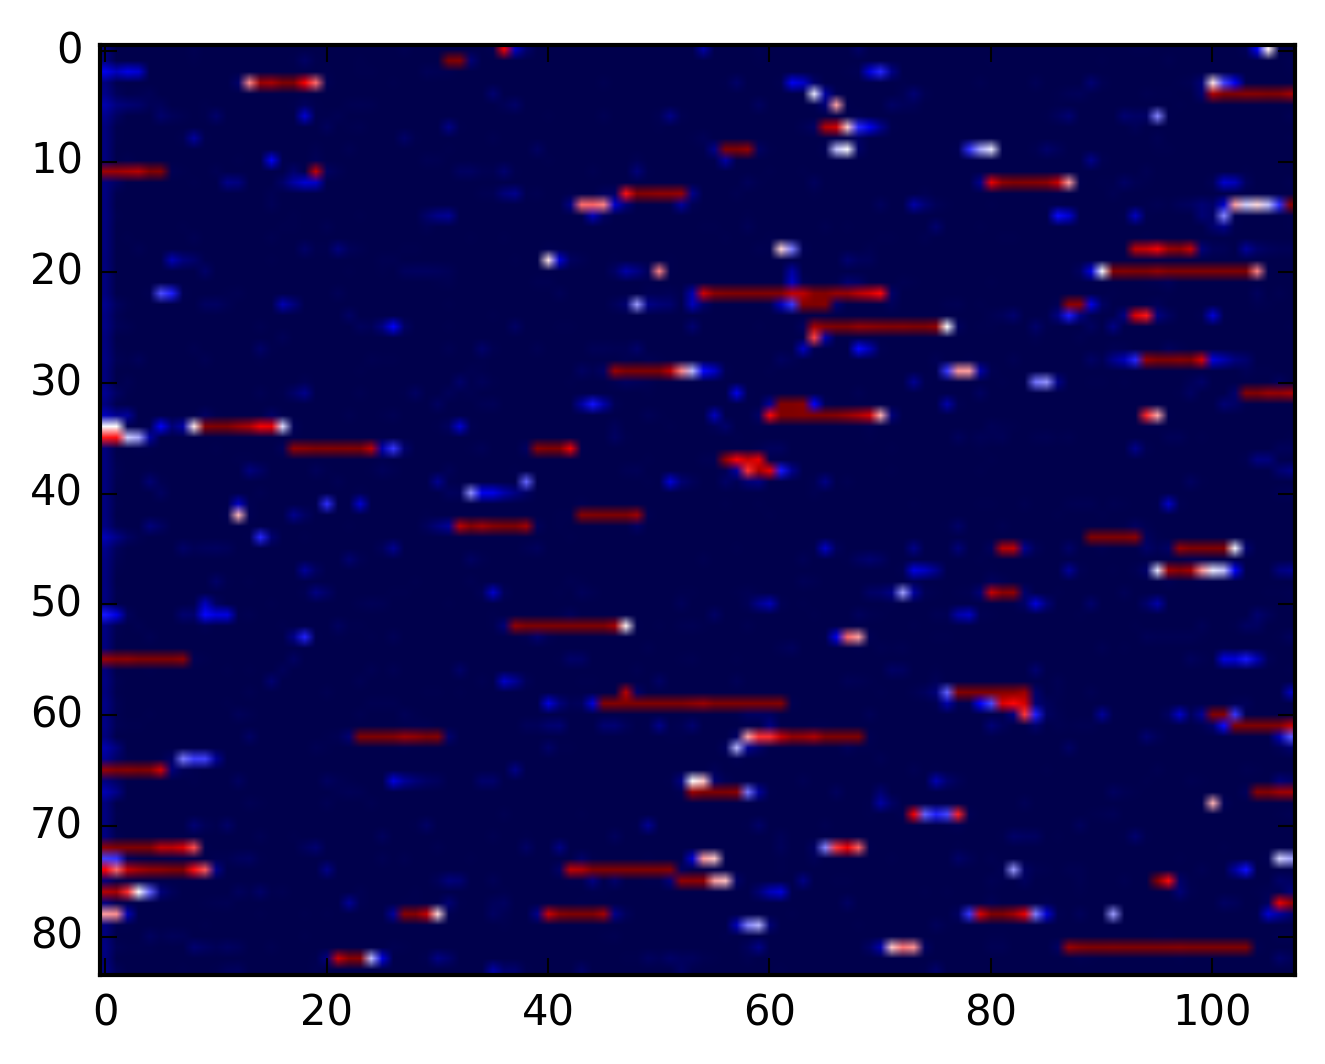
\includegraphics[width=60mm]{predicted_AEM.png}
}
\end{tabular}
\caption{Latent States ($X$) Predictions}
\label{fig:X_prediction}
\end{figure*}

\subsection {Comparative Analysis}  

The parameter estimation results by Gibbs sampling with 500 iterations and GBW algorithm with 15 iterations is shown in Table \ref{tab:para}. Notice that Gibbs sampling implemented in the experiments burns in half of the total number of iterations.  Both algorithms result in similar parameter estimations. Generalized BW algorithm shows better performance than Gibbs sampling for less iterations (5-10 iterations for GBW, 500 iterations for Gibbs), while Gibbs sampling converges with less time (will be discussed in section Profiling and Optimization). Although as we will discussed in section Code Testing, Gibbs Sampling is subjective to prior choices, an excellent performance of GBW is even largely dependent on the initialization of parameters. If the initializations are chosen inappropriate, GBW may harm the result, which is the common disadvantage of EM algorithm.

\begin{table}[htpb]
\caption{Parameter Estimation}
\hspace*{-3.8cm}
\begin{tabular}{|l|c|c|c|c|c|c|c|c|c|c|c|c|c|c|c|c|}
\hline
\bfseries $\Theta$ & \bfseries $\xi$ &  \bfseries $\alpha$ & \bfseries $\beta$ & \bfseries $\gamma$ & \bfseries $\theta_{1,1}$ & \bfseries $\theta_{1,2}$ & \bfseries $\theta_{1,3}$ &\bfseries $\theta_{1,4}$ &\bfseries $\theta_{1,5}$ &\bfseries $\theta_{1,6}$ &\bfseries $\theta_{0,1}$ &\bfseries $\theta_{0,2}$ &\bfseries $\theta_{0,3}$ &\bfseries $\theta_{0,4}$ &\bfseries $\theta_{0,5}$ &\bfseries $\theta_{0,6}$ \\  
    \hline
    Gibbs-500 & 0.133 & 0.009 & 0.016 &  0.223 & 0.666 & 0.597 & 0.683 & 0.471 & 0.596 & 0.638 & 0.207 & 0.196 & 0.315 & 0.230 & 0.416 & 0.067 \\\hline
    GBW-15 & 0.095 & 0.007 & 0.002 & 0.181 & 0.680 & 0.624 & 0.703 & 0.494 & 0.606 & 0.680 & 0.209 & 0.197 & 0.316 & 0.230 & 0.416 & 0.068 \\\hline
\end{tabular}
\label{tab:para}
\end{table}

\subsection{Application to Simulated Data Set}
\paragraph {Missing observed states imputation} Due to privacy of the participants, we do not have access to the original clinical data. The dataset we have at hand is already cleaned with missing values imputed. To mimic the real situation when students are too lazy to report the 6 symptoms everyday, we simulate from this data set a proportion of student-day combinations and set the observed states ($Y$) of those as missing. Meanwhile, we add an additional step in Gibbs Sampler loops to sample these observed states ($Y$) from Bernoulli distribution with certain probability ($\theta_1$ if infected, $\theta_0$ if not infected).
Since the actual number of students who have and also report these symptoms is sparse, the majority positions of Y are 0's. Therefore we are interested in whether our model commits type II error --  predicting none when the student truly has a symptom, and we compare the performances with missing y using FNR (False Negative Rate) as we have true value of Y for the predicted ones in this case. As we can see, FNR increases modestly with small missing rate, and dramatically when missing rate larger than 0.7. This is because the Y matrix is sparse and therefore the simulated missing are mostly 0’s as well. Setting those as missing does not affect our prediction much. However, when missing rate is as high as 0.8, we are losing valuable information by ignoring a considerable portion of 1’s as missing. 

\begin{figure}[htpb]
\centering
\subfigure[False Negative Rate]{
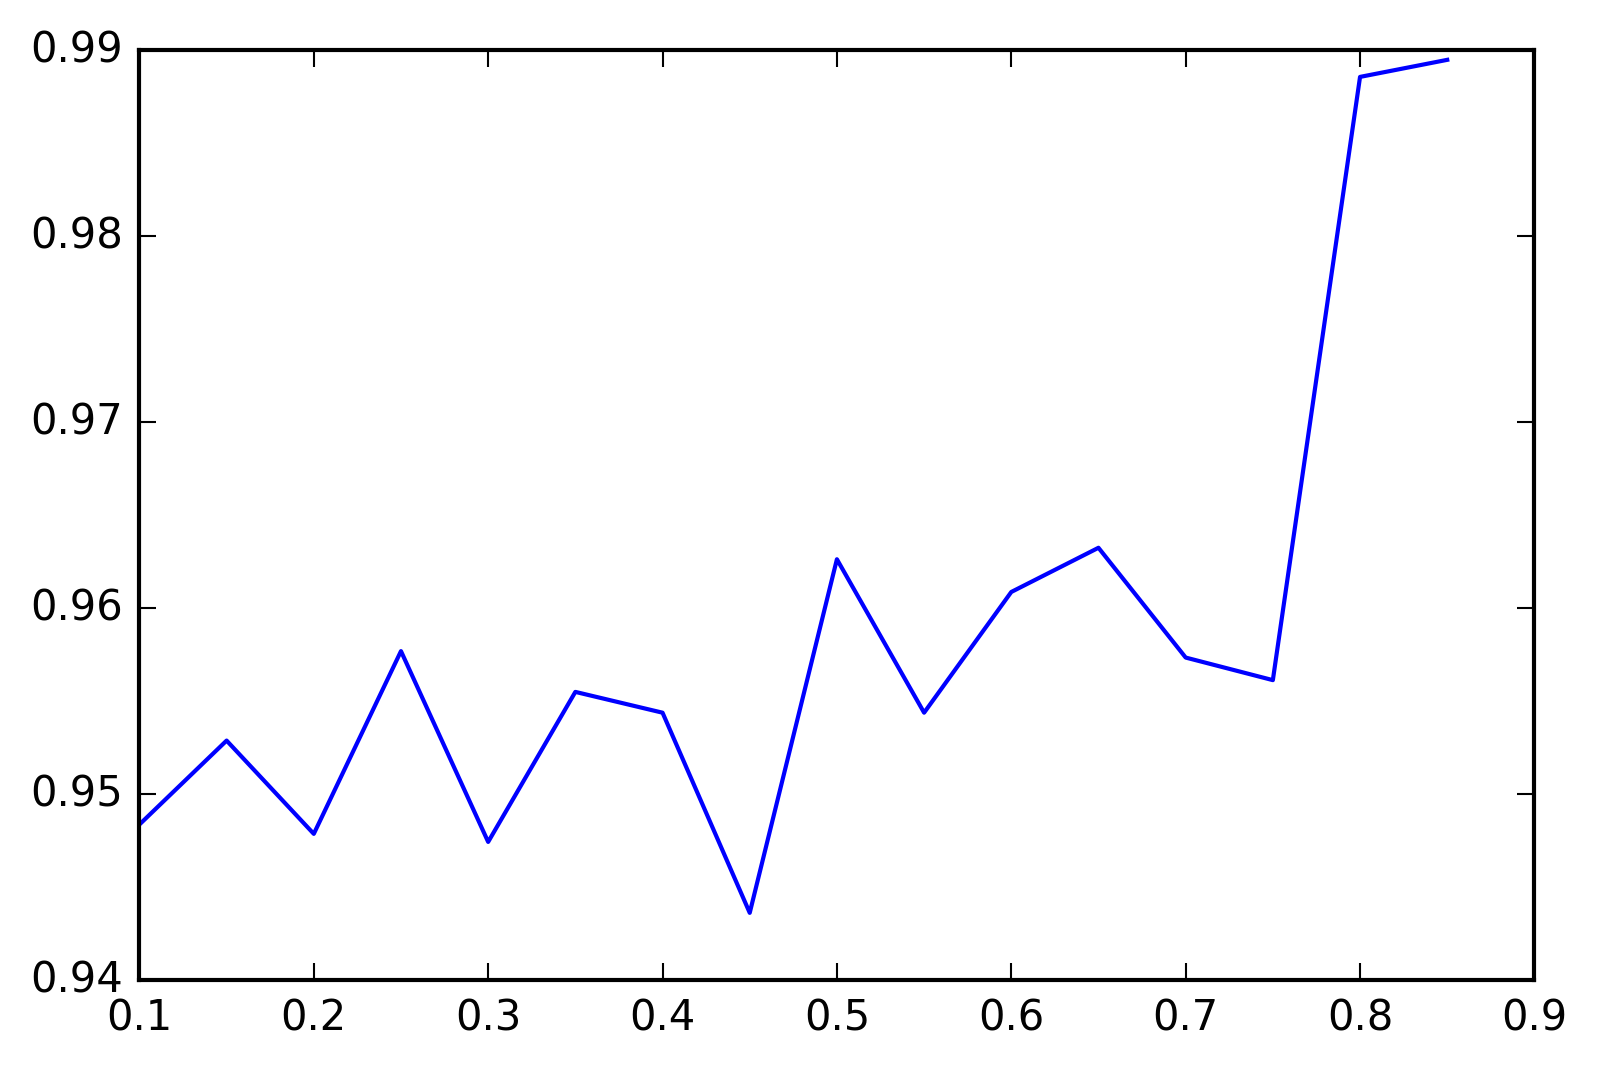
\includegraphics[width=70mm]{FNR.png}
}
\end{figure}


\paragraph {Latent states prediction with missing Y} Our explanation is also verified by the latent states prediction heat maps with missing values. When missing rate is 20\% or 40\%, the model achieves more or less the same result. When missing rate is 60\%, the model has more noise (light blueness indicating that the student still has a less than 0.5 probability of being infected). When missing rate is 80\%, the model is very unconfident in predicting anyone as infected

\begin{figure*}[h]
\hspace{-3cm}
\begin{tabular}{ccc}
\subfigure[20\% missing]{
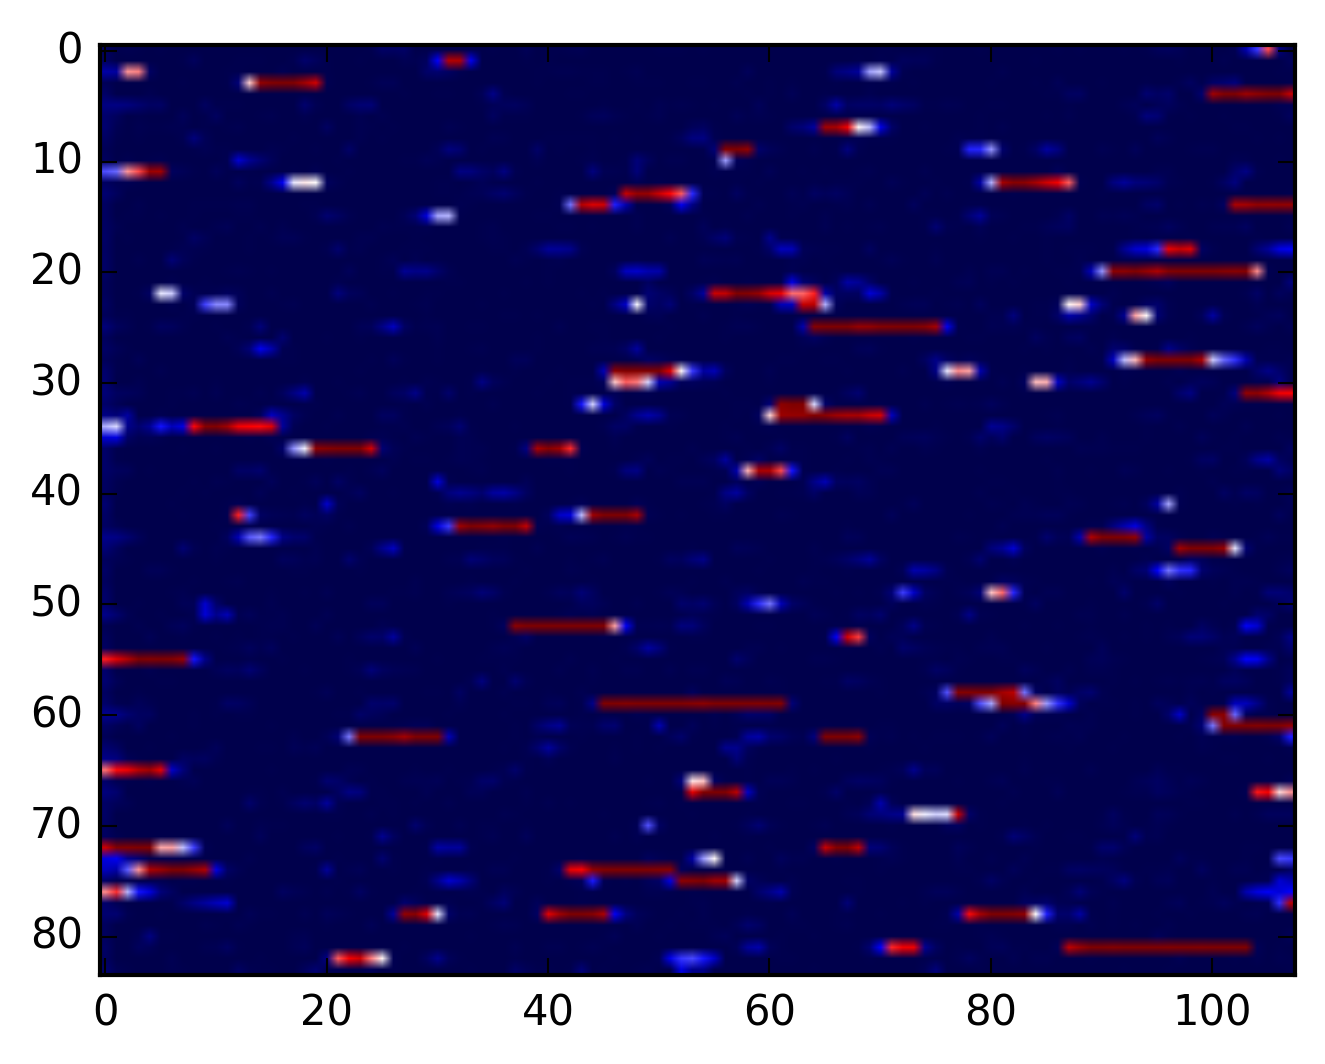
\includegraphics[width=60mm]{missing02.png}
} &
\subfigure[40\% missing]{
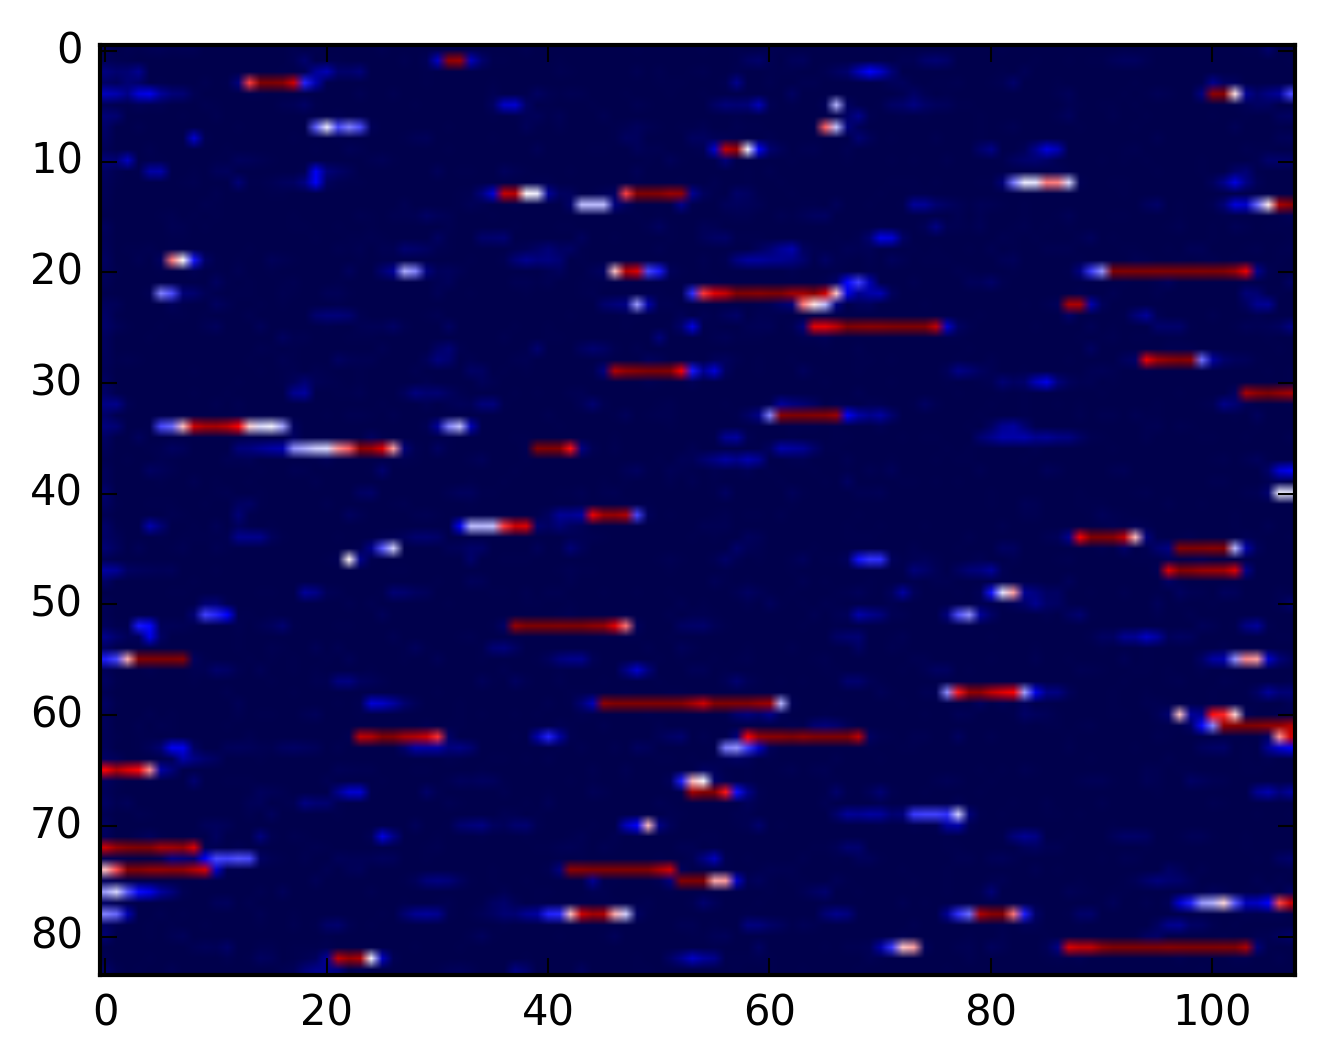
\includegraphics[width=60mm]{missing04.png}
} &
\subfigure[60\% missing]{
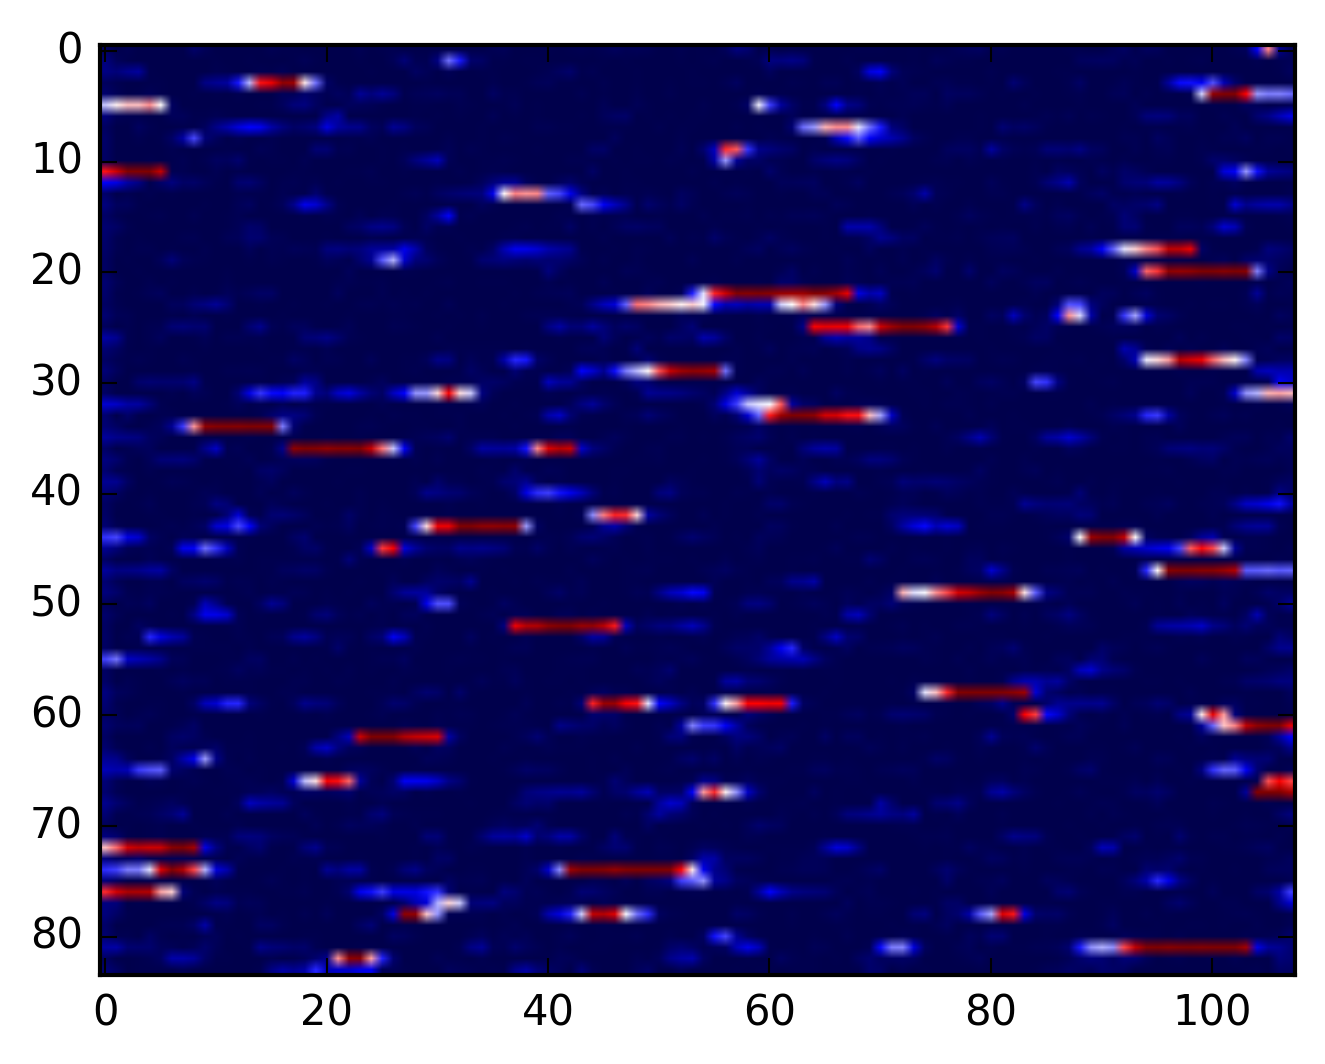
\includegraphics[width=60mm]{missing06.png}
} \\
\subfigure[80\% missing]{
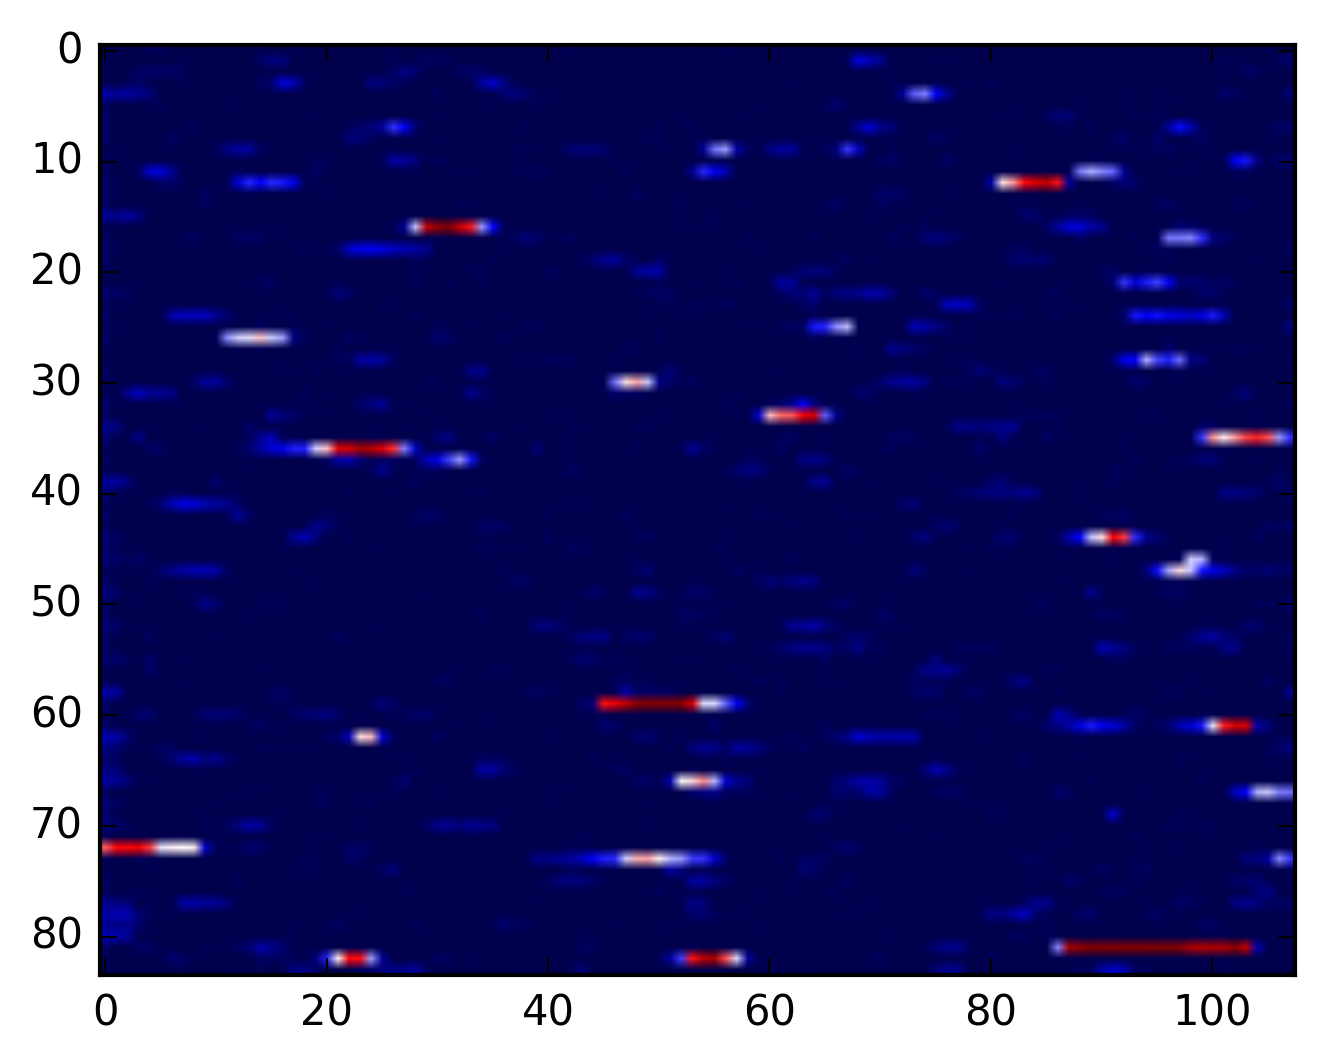
\includegraphics[width=60mm]{missing08.png}
} &
\subfigure[0 missing]{
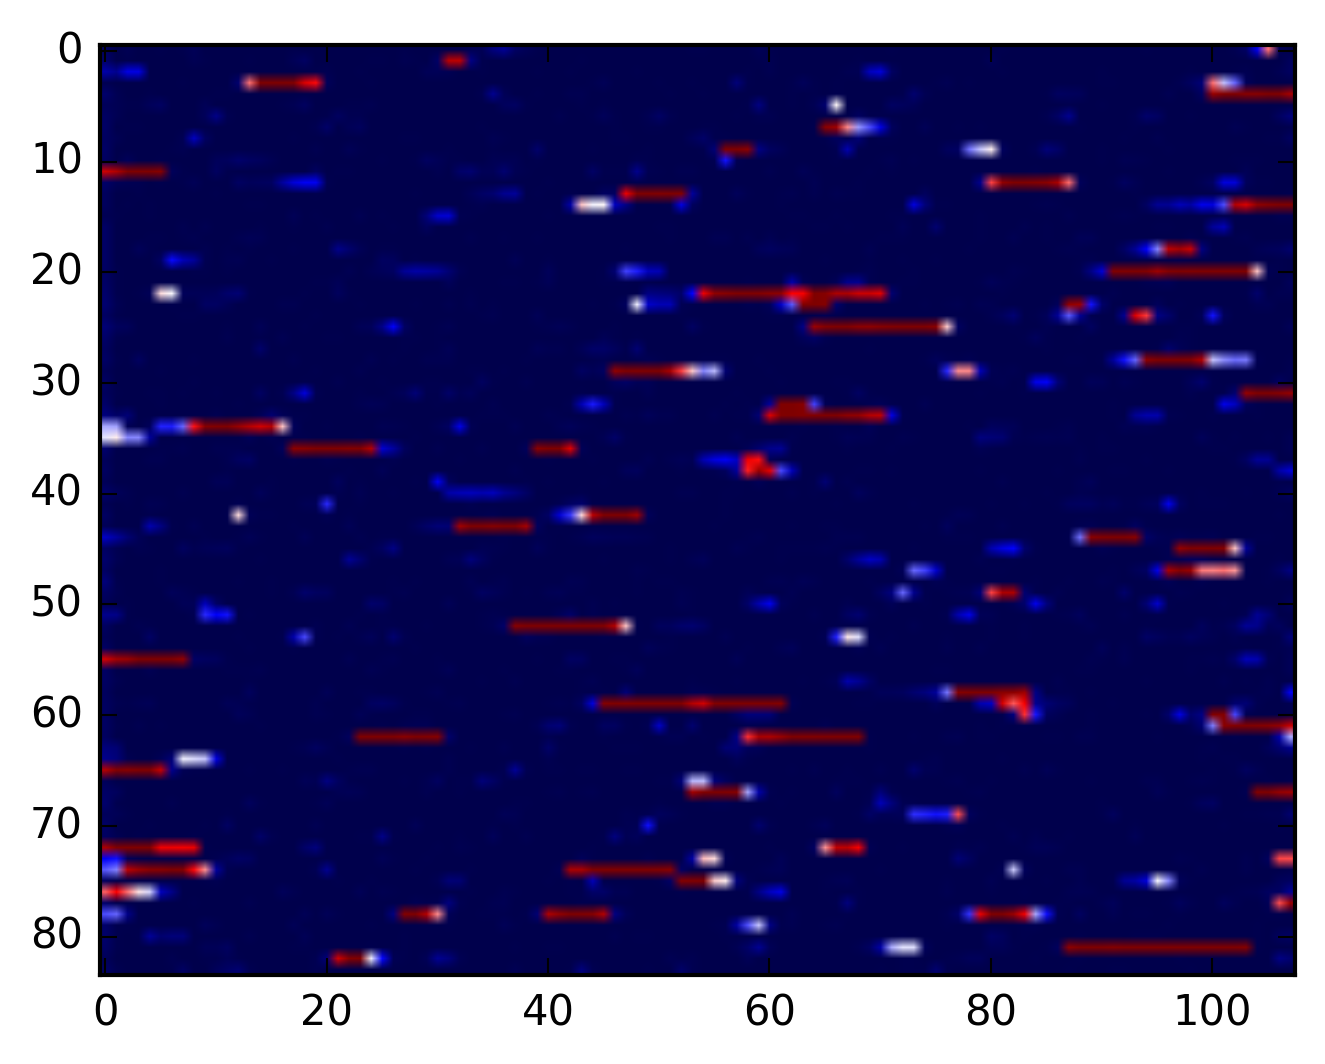
\includegraphics[width=60mm]{predicted.png}
} &
\subfigure[True Latent States]{
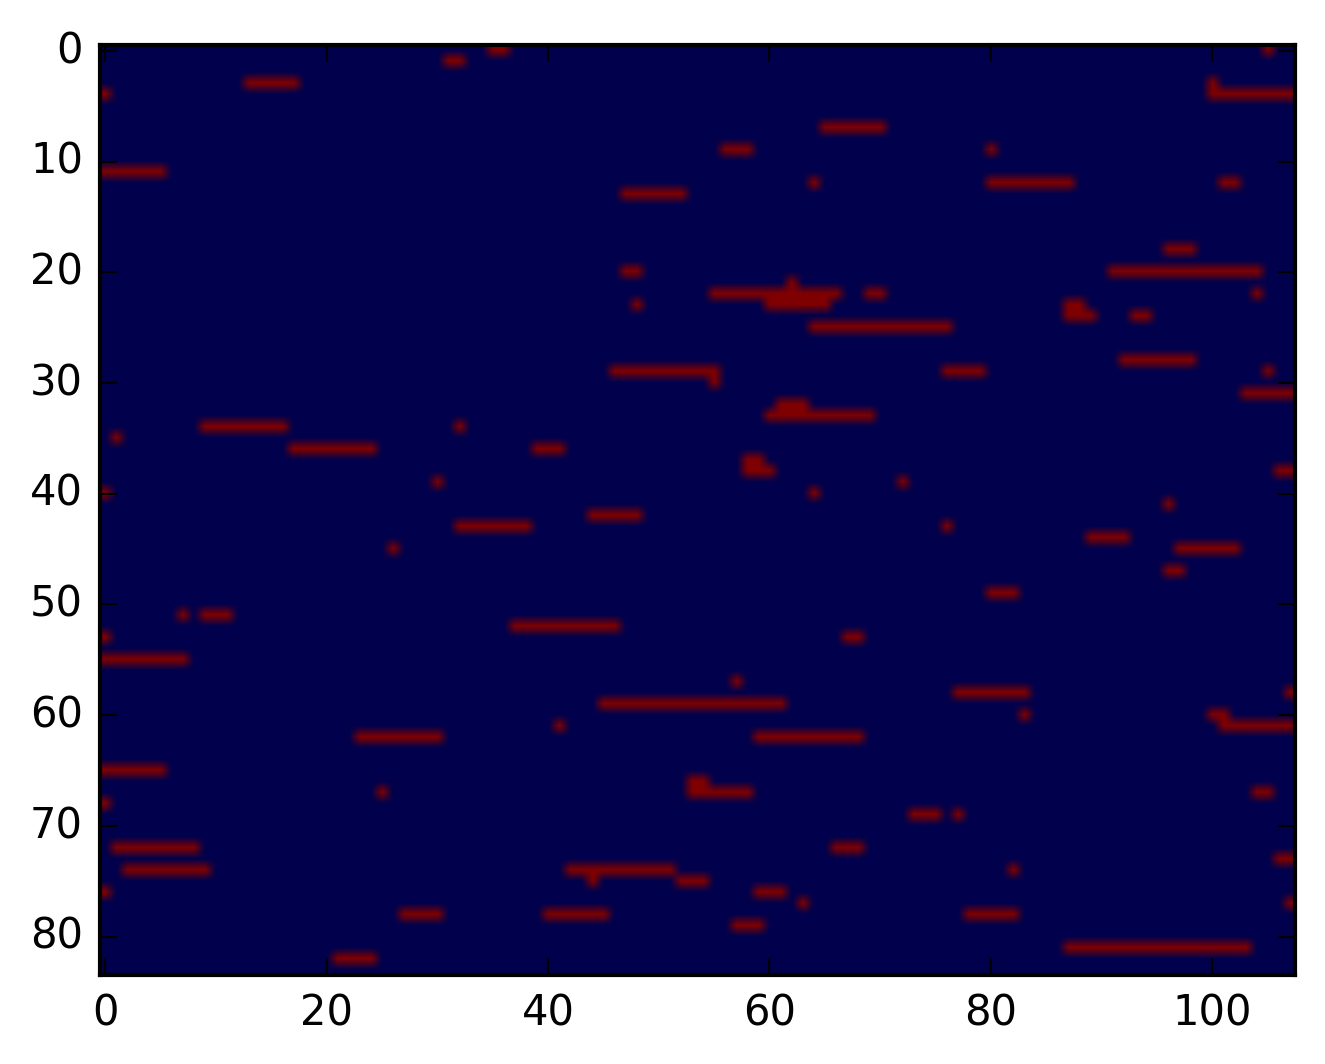
\includegraphics[width=60mm]{true.png}
}
\end{tabular}
\caption{Prediction of $X$ with different $Y$ missing rates.}
\label{fig:missing}
\end{figure*}



\section{Profiling and Optimization}

In this part, we performed both profiling and optimization on the Gibbs Samplers and Generalized Baum-Welch algorithm.


\subsection{Profiling and Optimization for Gibbs Sampler}

\subsubsection{Naive Version}

For the Gibbs Samplers, we wrote our algorithm in numpy for large parts, but left the core matrix multiplication function NumPreInf in nested for loop form for the further optimization. Our first naive version code consisted of one main function and seven small functions. 

\begin{python}
p = pstats.Stats('work_naive.prof')
p.sort_stats('ncalls').print_stats(10)
pass
\end{python}
\begin{figure}[htpb]
\centering
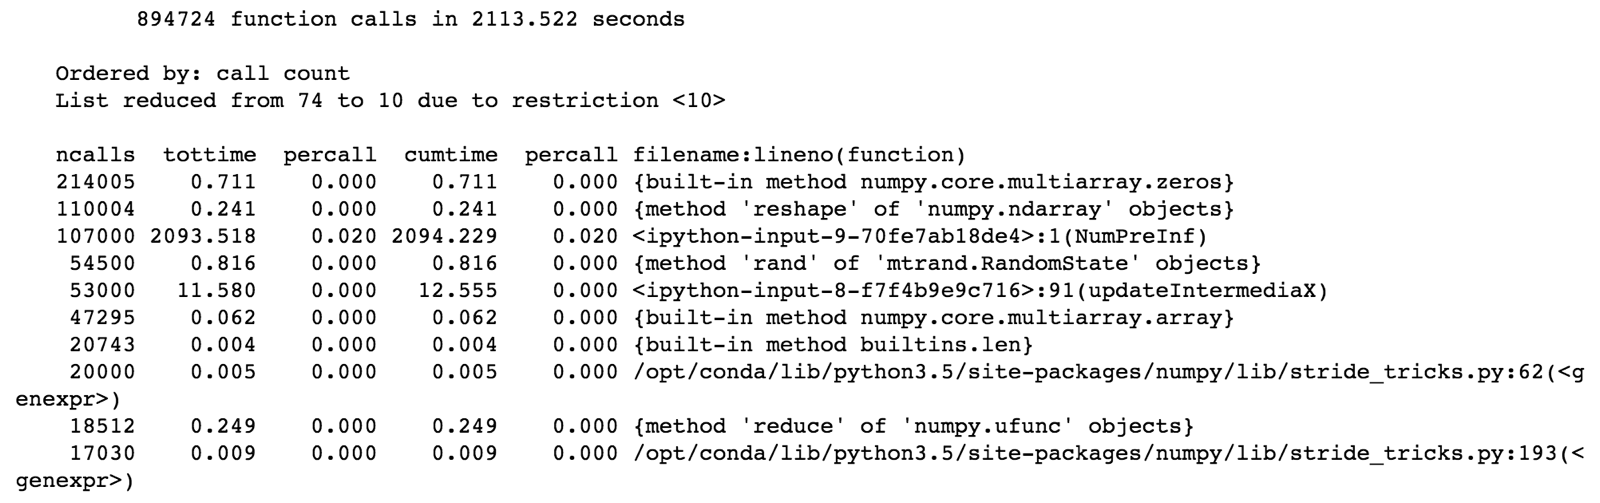
\includegraphics[width=160mm]{Gibbs_naive.png}
\end{figure}

We used over 2000 second to complete profiling on this naive version and found the NumPreInf function taking up almost all the running time. From this result, it was infeasible to write the whole code in for loop, and we were focus on optimizing NumPreInf function by serval methods.

\subsection{JIT Optimization}
we just put the JIT decorator on the chunk of NumPreInf function, and the total running times was reduced to 16.169 seconds.
\begin{python}
p = pstats.Stats('work_jit.prof')
p.sort_stats('ncalls').print_stats(10)
pass
\end{python}
\begin{figure}[htpb]
\centering
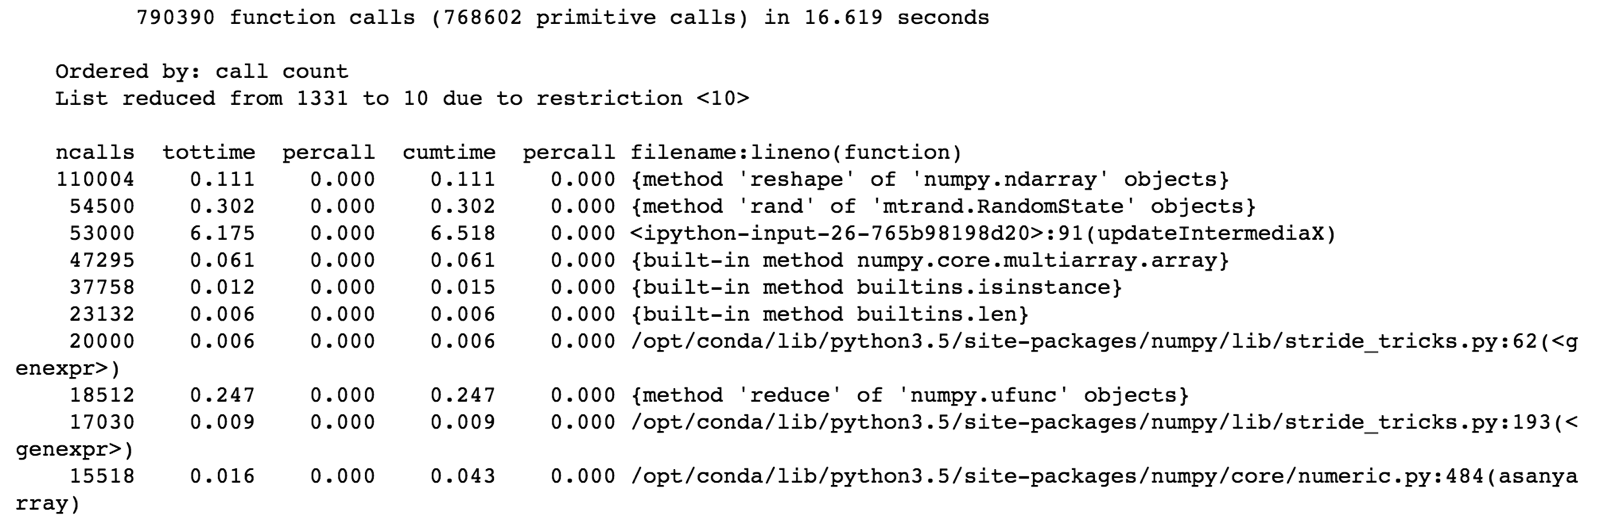
\includegraphics[width=160mm]{Gibbs_jit.png}
\end{figure}

\subsection{Cython Optimization}
Second, we re-wrote this function into Cython format, and the total running times was 16.545 seconds.
\begin{python}
p = pstats.Stats('work_cython.prof')
p.sort_stats('ncalls').print_stats(10)
pass
\end{python}
\begin{figure}[htpb]
\centering
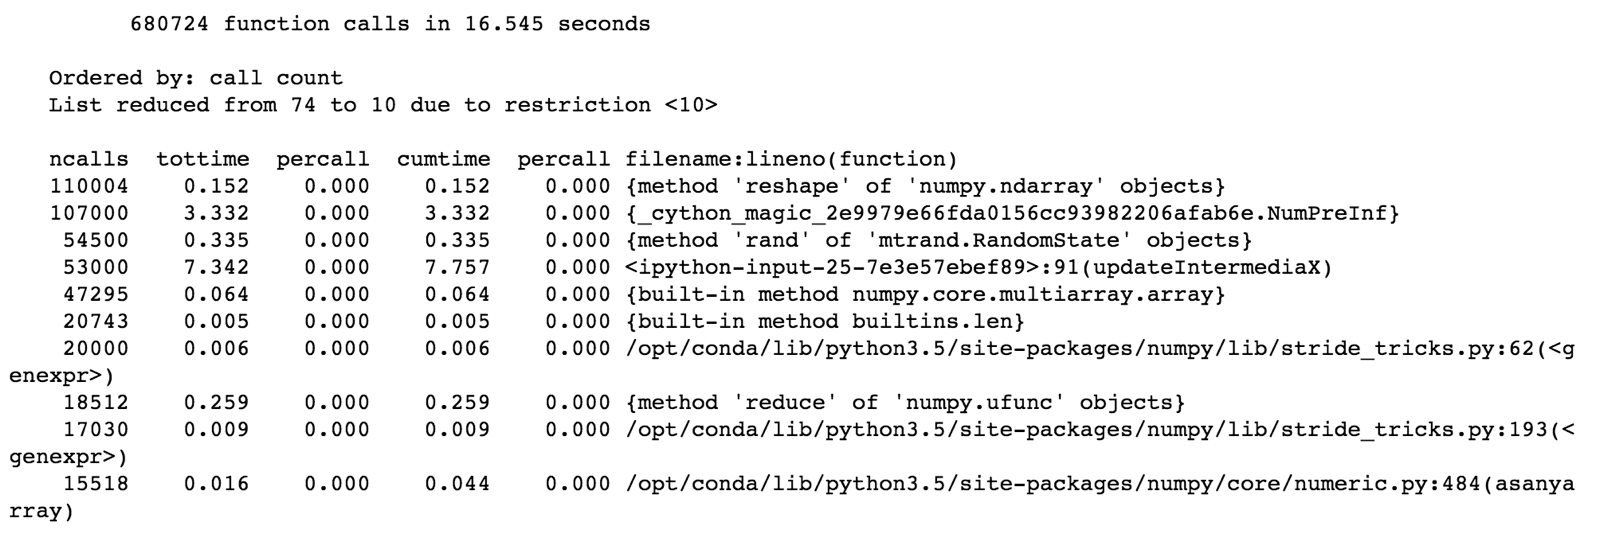
\includegraphics[width=160mm]{Gibbs_cython.png}
\end{figure}


\subsection{Broadcasting with Numpy}
Third, we used numpy broadcasting to replace the nested for loops which reduced the total running time to 15.517 seconds.
\begin{python}
p = pstats.Stats('work_numpy.prof')
p.sort_stats('ncalls').print_stats(10)
pass
\end{python}
\begin{figure}[htpb]
\centering
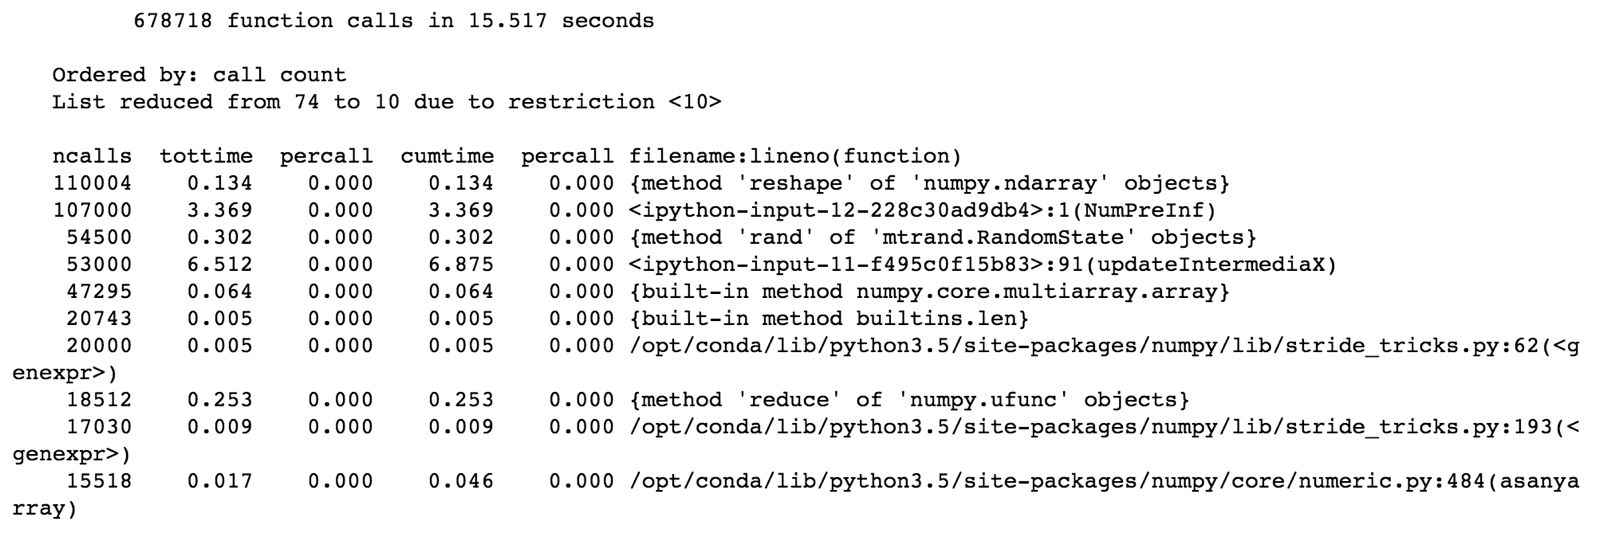
\includegraphics[width=160mm]{Gibbs_numpy.png}
\end{figure}

\subsection{Merging Small Functions}
All of these methods produced similar optimization results which greatly decreased the total running time. In order to further optimize the running time, we tried to reduce the total number of function calls by integrating small functions into the main function. After re-constructing our algorithm, we only left NumPreInf function in numpy version and one big function `Gibbs Whole`. By doing so, we reduced the total numbers of function call from 678,718 times to 524,723 times, which further improved the total running time to 10.767 seconds.

\begin{python}
p = pstats.Stats('Gibbs_GCHMM.prof')
p.sort_stats('time', 'cumulative').print_stats(10)
pass
\end{python}
\begin{figure}[htpb]
\centering
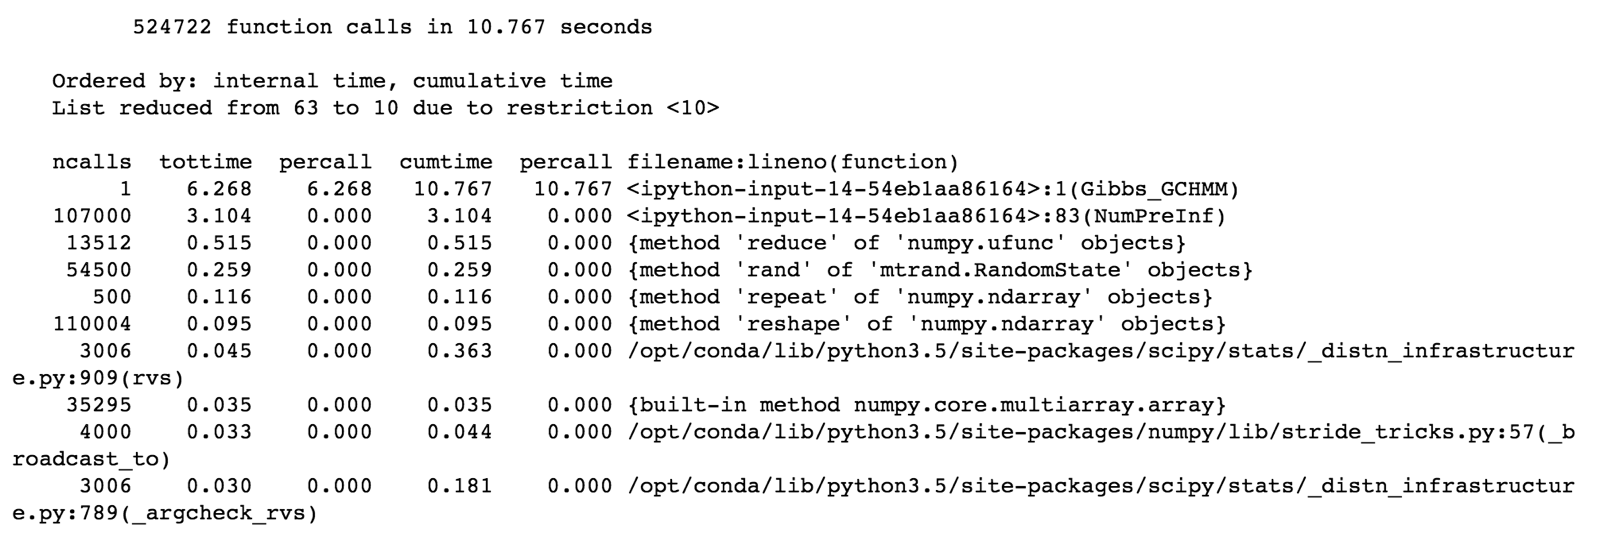
\includegraphics[width=160mm]{Gibbs_GCHMM.png}
\end{figure}

\subsection{Comparison Table for Gibbs Sampling}
Below is a comparison table for the different algorithms mentioned above.
\begin{figure}[htpb]
\centering
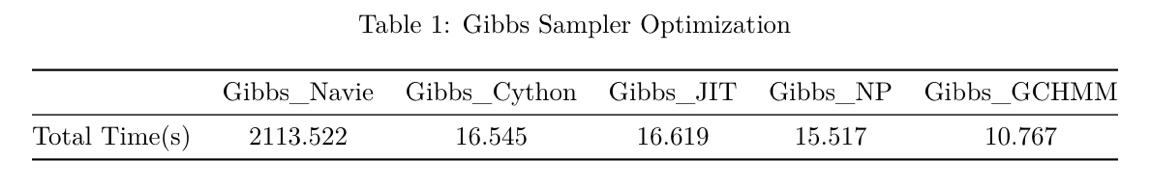
\includegraphics[width=120mm]{Gibbs.png}
\end{figure}

\subsection{Profilling and Optimization for Generalized Baum-Welch Algorithm}
For the generalized Baum-Welch algorithm (i.e., approximate EM belief propagation, AEMBP), we directly wrote whole algorithm in numpy with many broadcastings, since from the experience of the Gibbs Sampler, we found the numpy broadcasting was outperform than JIT and Cython. In addition, the generalized Baum-Welch algorithm is too complex to write in for loops first, which may take incredible long time to run the naive version. Based on the pre-optimized the algorithm, we did optimization by removing many redundant calculations. 

\begin{python}
p = pstats.Stats('AEMBP.prof')
p.print_stats(10)
pass
\end{python}
\begin{figure}[htpb]
\centering
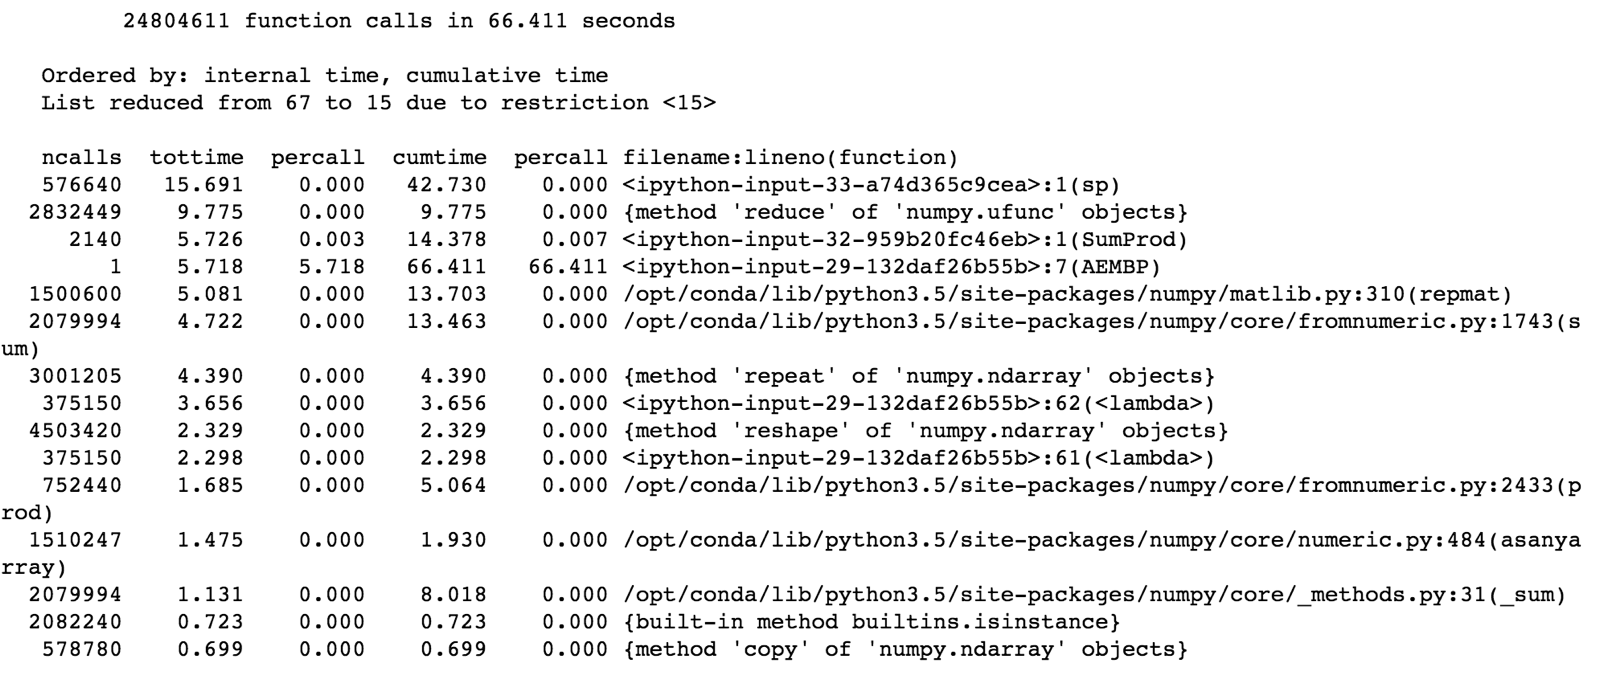
\includegraphics[width=170mm]{AEMBP_profile.png}
\end{figure}

\subsubsection{Pre-computing - Reduce Redundant Iterations}
After profiling the numpy version code, we found the np.sum in fGX, SumProd, and sp functions cost lots of time. After exploring our code, we found that we lost much efficiency on calculating np.sum of different length lists by 1 axis in nested for loops. Thanks to the special property of our network which the maximum degree of node is 11, it was feasible to compute all np.sum of different length lists by 1 axis, which depended on degree of node outside the function and passed it as a parameter into our function. By doing so, we reduced the total function calls from 24,804,611 times to 24,109,445 times for 5 iterations, which shortened the total running time from 66.411 seconds to 56.983 seconds. If our algorithm is running a large data set which requires a large numbers of iteration to converge, our optimization will be very promising and saving lots of running time.

\begin{python}
p = pstats.Stats('AEMBP_GCHMM.prof')
p.sort_stats('time','cumulative').print_stats(15)
pass
\end{python}
\begin{figure}[htpb]
\centering
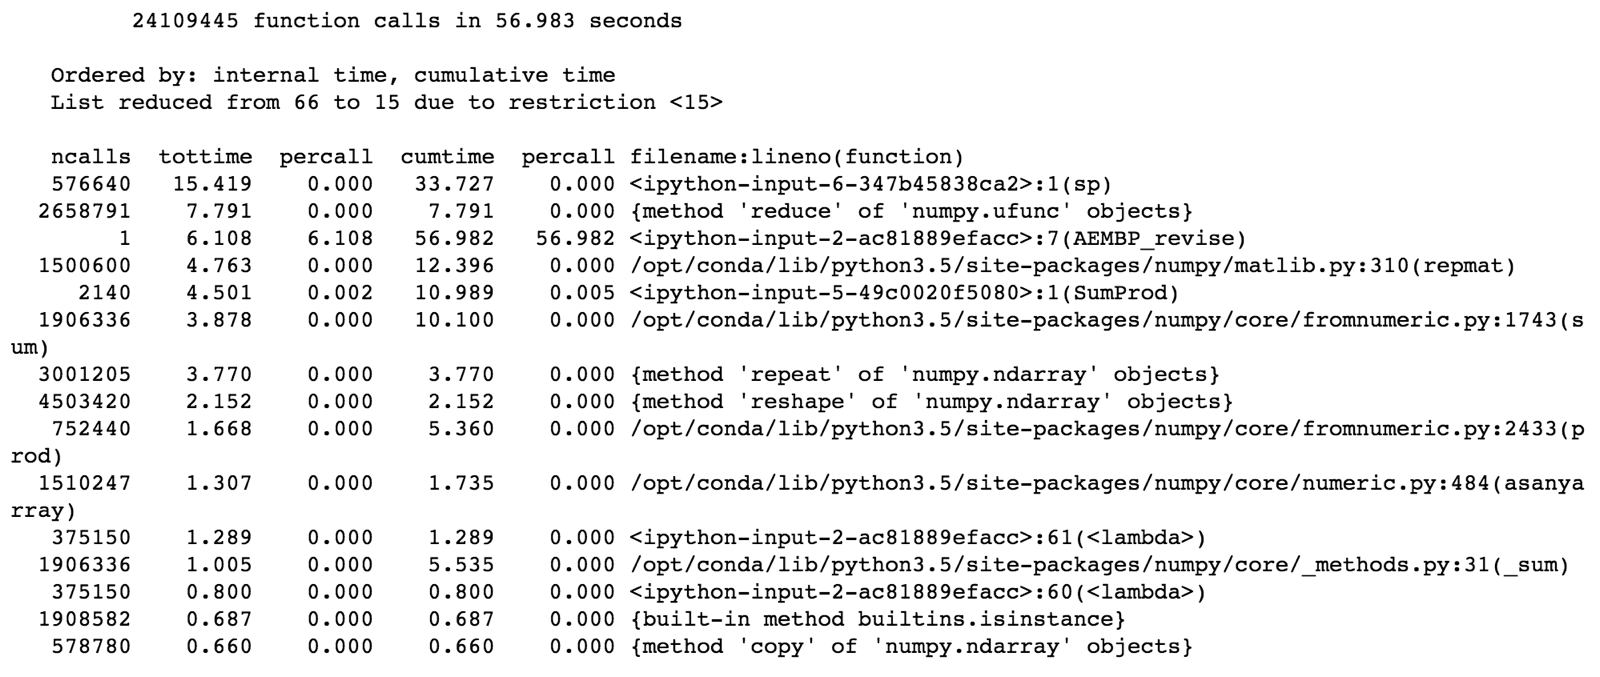
\includegraphics[width=160mm]{AEMBP_revise_profile.png}
\end{figure}

\subsection{Comparison Table for Generalized Baum-Welch}
Below is a comparison table for the different algorithms mentioned above.
\begin{figure}[htpb]
\centering
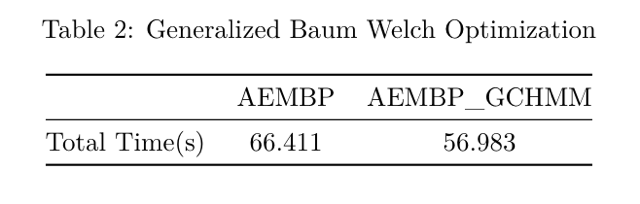
\includegraphics[width=90mm]{AEMBP.png}
\end{figure}


\section{Code Testing}

\subsection{Test on Prior Choices}

\begin{python}
assert(ap < bp & aa < ba & ab < bb & ar < br & a1 > b1 & a0 < b0)
\end{python}

Remember our priors elicitation:

Priors on emission parameters:
$\theta_0 \sim \text{Beta}(a_{0}, b_{0}), \theta_1 \sim \text{Beta}(a_{1}, b_{1})$

Priors on transition parameters:
$\alpha \sim \text{Beta}\left ( a_{\alpha},b_{\alpha} \right ), \beta \sim \text{Beta}\left (a_{\beta}, b_{\beta}\right ), \gamma\sim \text{Beta}\left (a_{\gamma}, b_{\gamma}\right ), \xi \sim \text{Beta}(a_{\xi}, b_{\xi})$

We set these priors to be:
$( a_{\alpha},b_{\alpha}) = (a_{\beta}, b_{\beta}) = (a_{\gamma}, b_{\gamma}) = (a_{\xi}, b_{\xi}) = (a_0, b_0) = (2, 5), (a_1, b_1) = (5,2)$ when actually implementing the algorithm.

$\gamma$ stands for recovery probability if infectious at pervious time
$\alpha$ stands for probability being infected from some one outside networks
$\beta$ stands for probability being infected from some one inside networks
$\xi$ is the prior probability for a Bernoulli distribution of $X_{n,1}$, i.e., the probability that a student get infected on the first day. These are very small probability values, and therefore should have a left-skewed beta distribution. We used `assert` function to make sure these priors are on a reasonable scale.

$\theta_1$ is the probability of presenting a symptom under the condition that the student gets infected. It should be larger than $\theta_0$, the probability of presenting a symptom under the condition that the student did NOT get infected. The assertion is important as we tested on boundary conditions when $\theta_1$ and $\theta_0$ has symmetric beta prior, i.e., $(a_0, b_0) = (a_1, b_1)$, the resulting heat map shows label switching problem. The algorithm cannot determine which one stands for the probability of getting infected.

\begin{python}
assert(ap < bp & aa < ba & ab < bb & ar < br & a1 > b1 & a0 < b0)
\end{python}

\subsection{Unit test}

As we discussed in last section, the optimized code only involves the large function of `Gibbs`, and the small function `NumPreInf`, the latter is tested by an external file for unit testing. The correctness is ensured by showing the function results in an unique value (of a 1-d numpy array).

\begin{python}
import unittest
import numpy as np

def NumPreInf(Xt, Gt):
    return ((Gt + Gt.T) > 0) @ Xt
    
class TestUM(unittest.TestCase):
 
    def setUp(self):
        pass
 
    def test_matrix(self):
        self.assertEqual( NumPreInf(np.array([1,0]), 
                                    np.array([[0, 1],
                                              [0, 0]])).all(), 
                          np.array([0,1]).all())

if __name__ == '__main__':
    unittest.main()
\end{python}

\begin{python}
wl-10-190-96-203:Desktop Emily$ python test.py 
.
----------------------------------------------
Ran 1 test in 0.000s

OK
\end{python}

\section{Conclusion} 
In this project, we implemented the two algorithms Gibbs sampling and Generalized Baum-Welch using approximate EM belief propagation to model the spread of infection within small community. In the actual dynamic social network data, maximum degree of $G_{84\times84\times107}$ is bounded by constant $M=11$, meaning that the number of connections per student per day cannot exceed 11. Several methods have been used to make the GCHMM implementation code faster, such as removing redundant calculations by converting 0 to 11 into binary sequence outside the function. However, the computation complexity is bounded by the maximum number of node in the graph.  If the maximum number of node is allowed to be even larger, the computation complexity will grow drastically. The boundary condition is a limitation to both the model setup and computation efficiency. In spite of that,  Graph-Coupled HMMs is still a popular choice and has already been wrapped up in mobile application to model flu diffusions.


\subsubsection*{Acknowledgments}

The author would like to thank \textbf{Kai Fan} for helpful discussions.  

\bibliographystyle{plain}
\small {\small{
{
\bibliography{reference}
}
}

\end{document}
